\documentclass[]{article}
\usepackage{fullpage}
\usepackage[authoryear]{natbib}
\usepackage{setspace}
    \doublespacing
\usepackage{hyperref}
\hypersetup{
    colorlinks,
    citecolor=black,
    filecolor=black,
    linkcolor=cyan,
    urlcolor=cyan
}
\usepackage{amssymb,amsmath}
\usepackage{bm}
\usepackage{dcolumn}
\usepackage{booktabs}
\usepackage{url}
\usepackage{tikz}
\usepackage{todonotes}
\usepackage[utf8]{inputenc}
\usepackage{graphicx}
\usepackage{longtable}
\usepackage{todonotes}
\usepackage{lscape}
\usepackage{float}
\usepackage[margins]{trackchanges}
\addeditor{MH}
\addeditor{CG}
\usepackage{subfig}
\captionsetup{belowskip=12pt,aboveskip=4pt}


\title{Measuring Real-time Perceptions of Financial Market Stress}
\author{Christopher Gandrud \\ \emph{City University London} \\ \emph{Hertie School of Governance}\footnote{Please contact Christopher Gandrud
(\href{mailto:gandrud@hertie-school.org}{\nolinkurl{gandrud@hertie-school.org}}).
Thank you to Ronen Palan for helpful comments, as well as Christian Franz and Sahil Deo for early research assistance. Our research is generously supported by the Deutsche Forschungsgemeinschaft. All data and replication material can be found at:
\url{https://github.com/christophergandrud/EIUCrisesMeasure}.}
\and
Mark Hallerberg \\ \emph{Hertie School of Governance}}

\begin{document}

\maketitle

\begin{center}
    \textbf{Working Draft \\ In preparation for the APSA 2015 Annual Conference, San Francisco}
\end{center}

\begin{abstract}
    Comparative quantitative research into the causes, responses to, and effects of banking crisis uses two series of crisis data: \cite{Reinhart2009,ReinhartRog2010} and Laeven and Valencia \citeyearpar[and their predecessors]{laeven2013}. While these data sets provide broad coverage, the measures they code have several shortcomings. They are constructed post hoc and so tend to be biased towards severe crises and away from circumstances where governments effectively calmed emerging trouble. They suffer from clear selection bias. Because they are simple dichotomous indicators of financial crisis, they do not indicate crisis severity. Our goal in this paper is to create a measure that is accurate, reliable, comparable across countries, and includes information about crisis severity. We use a kernel principal component analysis (PCA) of Economist Intelligence Unit (EIU) monthly country reports to develop a new real-time and continuous measure of perceived banking system stress. We refer to this measure as the EIU Perceptions of Financial Market Stress (FinStress) Index. We not only develop a novel indicator of financial market stress, but also make a contribution to the wider political science and finance literatures on measurement by demonstrating how kernel PCA can be used to efficiently summarise vast quantities of qualitative texts into useful continuous cross-sectional time-series indicators. Finally, we provide an application of our measure demonstrating that governments reveal more of the debt created by responding to financial market stress when they are electorally safe.

\end{abstract}


Why and how do politicians respond to financial market stress? What are the political consequences of crises? These questions have attracted considerable attention following the 2007-2009 crisis, and earlier late-1990s Asian financial crisis. However, most research on these topics lacks a crucial variable: a real-time indicator of the level of financial market stress that policy-makers perceived. To understand why politicians made a given choice in response to financial market stress, we need a measure of the conditions that existed as perceived in real-time. The literature on the political responses to and effects of financial crises has relied on two measures of financial crisis--\cite{Reinhart2009,ReinhartRog2010} or Laeven and Valencia \citeyearpar[and their predecessors]{laeven2013}. These measures are post hoc binary assessments of crisis occurrence and therefore are particularly lacking for studying politicians' responses to financial market stress.

In this paper, we develop a new index of real-time perceptions of financial market stress. We create this variable using a kernel principal component analysis (PCA) of detailed qualitative data, namely monthly Economist Intelligence Unit (EIU) reports. We call it the EIU Perceptions of Financial Market Stress (FinStress) Index. This measure has several advantages over the popular measures of crisis. It is continuous instead of dichotomous, and it allows researchers to identify episodes of stress where policy-makers successfully avoided a full-blown crisis. We also make a contribution to the wider political science literature by showing how kernel PCA can be used to summarise vast quantities of qualitative texts into continuous cross-sectional time-series indicators.

We start the paper by explaining previous attempts to measure financial market crises and stress, as well as identifying areas where they could be improved. We then discuss the construction of the FinStress Index and assess its validity. We compare it to widely used previous measures of financial market stress that are based on both quantitative and qualitative data. We then document theoretically interesting variation in the Index, including how it differs across developed and developing countries and how it changes over time within countries. This index allows us to draw conclusions about how financial market conditions differ across countries and how perceptions of financial market stress change over the course of crises. We also provide an example of how the Index could be used in applied research on political budget cycles.

\begin{table}
    \caption{Comparison of Crisis Measures' Definitions}
    \label{comp_table}
    \begin{center}
        \begin{tabular}{m{3cm} | m{2cm} m{2cm} m{7cm}}
            Source & Measurement Level & Periodicity &  Definition of Financial Market Distress/Crisis \\
            \hline\hline
                Reinhart and Rogoff \citeyearpar[11]{Reinhart2009,ReinhartRog2010} & binary & annual & One of two types of events: (1) bank runs leading to closures, mergers, or public sector takeovers of one or more financial institution or (2) the closure, merger, takeover, or large-scale government assistant--at least three measures--of an important financial institution marking the start of a string of similar events.  \\
                Laeven and Valencia \citeyearpar[228]{laeven2013} & binary & annual & Meets two conditions: (1) significant sign of financial distress in the banking system and (2) significant banking policy intervention measures in response to significant losses in the banking system.  \\
                Romer and Romer \citeyearpar[3]{Romer2015} & ordinal (0 to 15 scale) & bi-annual & Hand-coded perceptions of funding problems and rising loan defaults in \emph{OECD Economic Outlook}  \\
            \hline
        \end{tabular}
    \end{center}
\end{table}

\section{Motivation}\label{motivation}

Knowing when crises started, when they ended, and how severe they were over their course is crucial for understanding how governments choose to respond to financial market distress, the fiscal costs of these responses, and the political outcomes. Researchers working on these issues rely on two data sources of cross-country information on when a country is facing a financial crisis--\cite{Reinhart2009,ReinhartRog2010} or Laeven and Valencia \citeyearpar[and their predecessors]{laeven2013}.

Please see Table \ref{comp_table} for the criteria these data sets use to code a given country-year as being in a crisis. Reinhart and Rogoff \citeyearpar[10]{Reinhart2009,ReinhartRog2010} classify counties as being in crisis when they experience at least one type of event: (1) one or more bank run, closure, merger, or public sector takeover and/or (2) closure, merger, takeover or large-scale public assistance of an important financial institution that marks the start of a string of similar events. Laeven and Valencia \citeyearpar[228]{laeven2013} take a similar approach, that nonetheless emphasizes public interventions. They classify a country-year as in crisis when there is both significant distress in the banking system \emph{and} policy-makers respond to the distress with significant interventions.

These indicators have been widely employed in the literature and are critical indicators for evaluating the political economy of financial crises. \cite{Keefer2007} and \cite{Rosas2006,Rosas2009} used earlier versions of the \cite{laeven2013} data set to identify periods of crises and to argue that electoral competitiveness affected the type of policy response, as well as in Keefer's case the overall costs of the crisis to taxpayers. \cite{Gandrud2013,Gandrud2014} and \cite{Kleibl2013} combine the two data sources to understand how financial regulatory structures are changed in response to crises. \cite{broz2013} takes a similar approach of integrating the data sets to find a ``partisan financial cycle'' where right-leaning pro-market governments implement policies that create economic booms, but also lead to crises. Voters then elect left-leaning governments to clean up afterwards. \cite{CrespoTenorio2014}, \cite{Chwieroth2013}, and \cite{Pepinsky2012} used the data sets in their research on the political effects of crises. \cite{CrespoTenorio2014} found that incumbents in countries with open capital markets are more likely to survive a crisis in power than incumbents in countries with closed capital markets. \footnote{For an additional review of the literature see \cite{GandrudHallerberg2015}, as well as tables \ref{LitRevTable} and \ref{LitRevTable2} in the Online Appendix.}

There are several redeeming qualities to these data sets. They come from detailed comparative work that identifies some key features of crises, including estimated fiscal costs. They also differentiate across different types of crises, such as exchange rate, inflation, and banking crises. Yet, there are a number of problems with these indicators for studying political behaviour. Crucially, crises are identified post hoc by researchers who know what happened after the fact. Financial market stress that policymakers successfully address, thus preventing a major crisis, is not included. Similarly, stress that a government temporarily dampens through unsustainable policy measures, only to flare up later, is not recorded. This makes it difficult to study why and how politicians respond to financial market stress. An additional issue is that the measures are dichotomous and so do not give any indication of how severe crises were. Having a dichotomous measure also means that measurement errors--incorrectly timing the start or end of a crisis--can strongly bias econometric model estimates.

There are large inconsistencies between the timing of crises in the \cite{laeven2013} and \cite{Reinhart2009} data sets \citep{Chaudron2014}. For example, Japan is labeled as having a crisis between 1997 and 2001 by the former, but between 1992 and 1997 by the latter. Furthermore, \cite{GandrudHallerberg2015} find that there are significant differences in crisis timing between different versions of the \cite{laeven2013} data. The measures are at yearly intervals, prohibiting sub-annual analysis. Finally, while the measures use fairly precise definitions of when a crisis started, reasons for dating the end of a crisis are either unstated as in the case of \cite{Reinhart2009} or are ad hoc. Laeven and Valencia \citeyearpar[footnote 19]{laeven2013} determine that a crisis has concluded when real GDP and real credit growth are positive for two years, or five years have elapsed from the crisis start year.

\cite{Romer2015} attempted to address many of the problems in the \cite{Reinhart2009} and \cite{laeven2013} data sets by manually
classifying 24 countries on a 16 point scale of the cost of
credit intermediation. They code countries using information from the OECD's semi-annual \emph{Economic Outlook} reports from 1967 to 2007. Relying on contemporaneous reports allows for the construction of a real-time measure of credit market distress. This would allow us to examine policy choices that head off trouble or unsustainably prolong brewing difficulties. Their  continuous measure gives an indication of distress intensity.

However, their approach is also limited in a number of key ways. First, they are necessarily confined to the relatively small sample of OECD countries. Second, their measure is laborious and costly to create and update. Even if there were a more encompassing corpus of texts than the OECD \emph{Economic Outlook}, actually applying the method would be very costly. Third, relying on human coders introduces well-known problems of inter-coder reliability and unreproduciblity \citep{Minhas2015}.

Others have attempted to create measures of national banking system fragility and crisis using quantitative accounting and economic data. The finance literature relies on a statistical quantity know as Z-Scores. The concept was originally developed to assess firm solvency \cite{roy1952}. In the banking context, it is often used to measure national financial system fragility. This is useful for examining how banking system structure and policies affect the probability of bank-specific and financial system difficulties \citep[e.g.][]{beck2013bank,vcihak2010islamic,laeven2009bank,uhde2009}. Though there are various ways to calculate this measure \citep[73]{Lepetit2013}, in general bank accounting information--assets, equity, and return on assets--is used to create an inverse measure of the probability that a country's banking system is `insolvent'.

Another approach to measuring crises, though not necessarily crises confined to the banking sector, is to classify periods below a pre-specified output gap as being in crisis. For example, in his examination of reforms in response to economic crises, including financial crises, Galasso determines a crisis to be when the output gap falls below the 90 percentile in his sample \citeyearpar[154]{galasso2014}. Other work, notably \cite{laeven2013} and \cite{Reinhart2009} examine the output gap as a consequence of crisis, rather than the crisis itself.

There have been a number of recent innovations to the measurement of banking system stability using quantitative data. Building on \cite{vonHagen2007}, \cite{Jing2015} developed an index of money market pressure based on changes in short-term interest rates and stocks of central bank reserves. However, this measure conflates distress and policy responses and assume that central banks across countries use the same reaction function to increase demand for liquidity. \cite{Rosas2009} developed a dynamic latent trait model of banking system distress. His measure relies on nationally reported data to the IMF's International Financial Statistics (IFS). \cite{GandrudCopHal2015} show that reporting to the IFS is very uneven across countries and time. They indicate that decisions to report data to the IFS could be endogenous to political events, complicating attempts to use IFS data to date crisis occurrence and severity. Furthermore, as \cite{KayserLeininger2015} show, people make decisions based on contemporaneously available information, but researchers attempting to understand their behaviour often use data that has been significantly updated after the fact. Using revised IFS data will give an inaccurate impression of the conditions that politicians believed they faced at the time. In addition, apart from Z-Scores--one version of which is available from the World Bank's Global Financial Development Database \citep{worldbank2013}--many of these quantitative measures have not been made publicly available.

\section{Creating the FinStress Index}

We overcome many of the problems that plague previous measures by using a new approach to estimate real-time perceptions of financial market stress. Our method uses kernel principle component analysis \citep{Scholkopf1998,lodhi2002,Spirling2012} of country reports from the \emph{Economist Intelligence Unit}\footnote{See \url{http://www.eiu.com/}. Accessed May 2015.} to create a monthly index for almost all countries from 2003 through 2011.\footnote{Our approach is broadly similar to \cite{Minhas2015} who use a supervised machine learning approach called support vector machines and United States State Department Country Reports on Human Rights Practices to classify countries according to dichotomous regime types. Our work is distinct in that kernel PCA of EIU reports allows us to develop a continuous measure of perceived financial market stress. Also, their supervised learning approach assumes that countries have been well classified by previous indicators, which they use to train the model. As discussed above, we are not confident that this is the case for financial crisis. Therefore, we use the unsupervised kernel PCA approach to establish new estimates.}

\subsection{Why the EIU?}\label{why-the-eiu}

The EIU compiles real-time, third-party assessments of financial market conditions reported monthly or, for a small subset of countries, quarterly. These reports contain both summaries of present and future economic conditions. They are also a channel through which this information is disseminated to public and private actors in many countries. Together, the reports create a large corpus (more than 20,000 texts from 1997 through 2011) of reports for more than 100 countries. The texts generally follow the same format and style and contain directly comparable assessments of economic conditions across the globe over a significant time span. In contrast, the OECD \emph{Economic Outlook} provides comparable reports for a very small number of wealthy countries on a bi-annual basis. As such, the EIU is preferable for creating a cross-country indicator of perceived financial market stress.

\subsection{Summarising financial market stress in the
EIU}\label{summarizing-financial-market-stress-in-the-eiu}

Our aim is to create an index that classifies financial conditions on a continuous more-stressed/less-stressed spectrum for as many country-months as possible. Therefore, we need an efficient way to summarise the vast quantity of information in the EIU reports along such a spectrum. To do this we first collected and processed the EIU texts. We then used kernel principal component analysis to place the texts onto a financial market stress spectrum. We rescaled the Index to ease interpretation.

\subsubsection{Text selection}\label{text-selection}

EIU reports assess many economic sectors within a country,
not just the financial sector. So, our first step was to select the portions of the EIU texts that contained relevant information about countries' financial systems. We automatically collected and parsed the reports from their original HTML format. We then extracted the portions of the texts--headers and paragraphs--that contained at least one of a number of keywords concerning financial markets.\footnote{The
  keywords included: \emph{bail-out}, \emph{bailout}, \emph{balance
  sheet}, \emph{balance-sheet}, \emph{bank}, \emph{banks},
  \emph{banking}, \emph{credit}, \emph{crunch}, \emph{default},
  \emph{finance}, \emph{financial}, \emph{lend}, \emph{loan},
  \emph{squeeze}. These keywords are adapted
  from those used by \cite{Romer2015} and are intended to
  select passages that discuss credit market conditions.} Due to a significant change in the reports formatted in 2003, we also
selected only texts from 2003 in order to maintain comparability across the time-series.

We then preprocessed the texts using standard techniques \citep[see][]{Grimmer2013}.\footnote{All preprocessing was done using the \texttt{tm} package \citep{tm2015} in R \citep{R-cite}.} This involved removing common English words, such as `was' and `its'. The `stopword' list we used was from \cite{dhillon:modha:mlj01}. We stemmed the words so that different variants of the same word are represented by a common `stem'. This allowed us to work with a more manageable number of kernels.  We removed extra white space between the words, as well as punctuation and numbers. Finally, we dropped texts that included very few words (less than six). In practice, including these texts would have prevented the estimation of the kernel PCA model.

\subsubsection{Kernel Principal Component
Analysis}\label{kernel-principal-component-analysis}

Texts are frequently summarised using unordered `bags-of-words'
approaches, such as Latent Dirichlet Allocation. Clusters (bags) of `topics' within speeches or clusters of speeches around topics \citep[for a review see][]{Grimmer2013} are common results from these methods. We would like to preserve the order of the words in our texts and we would like to place the texts on a continuous scale that will be interpretable as a measure of perceived financial market stress. Many financial terms such as `credit growth' and `borrowing costs' are used in completely different senses depending on the adjectives that modify them. For example, `slowing credit growth' vs. `expanding credit growth' or `falling borrowing costs' vs. `increasing borrowing costs'. Likewise, adjectives can have very different implications for describing market conditions depending on the nouns that they modify. For example, `increasing' can indicate worsening conditions as in `increasing non-performing loans' or improving conditions as in `increasing lending'.  A
bags-of-words approach that treated each word as having meaning as an individual unit, rather than having meaning in ordered associations with other words, would not adequately capture common and radically different meanings in the EIU documents.

In order to address these issues we use kernel principal component analysis. This method was developed by \cite{Scholkopf1998} and \cite{lodhi2002}. \cite{Spirling2012} introduced it into political science. He used it to summarise changing trends in treaties between the US government and Native American groups. Kernel PCA allows us to extract structure from our likely high-dimensional EIU corpus \cite[6531--6537]{Zhang2010} while preserving word order.

Our unit of analysis is a sub-string kernel: a short sequence of letters\footnote{Following \cite{Spirling2012}, we used kernels with a length of five, i.e.~those that are five letters long. See also \cite{lodhi2002} who demonstrate that in English  string lengths between four and seven are often optimal.} that can be shared within and across words. Thus we can distinguish between two simple documents with the stemmed strings `slow credit' and `expand credit'. They share the five character kernels `credit, but differ on `slowc' and `pandc', among others. Using \cite{lodhi2002} we can summarise the similarity of these documents with the frequency distribution of five-length strings that they have in common--i.e. one--standardized by document length. We can find these pairs
for all of the documents in our corpus to create a kernel matrix. Finally, we can scale the documents using principal component analysis.\footnote{We conducted kernel PCA with the \texttt{kpca} function from the R package \textbf{kernlab} \citep{kerblabCite}.}

\subsubsection{Dimensionality}\label{dimensionality}

To determine the number of dimensions that best describe the data, we conducted a scree test, the results of which are shown in Figure \ref{scree_plot}. There is a clear `elbow' in the plot at component two. This suggests that the first component explains the most variation in the data. In the rest of the article we focus on the first dimension as the main dimension summarizing financial market stress. We examined a number of the other dimensions. However, these noticeably did not closely correspond to our priors about financial market stress based on previous indicators. Below we detail how the first component corresponds to our expectations of a valid measure of perceived financial market stress.

It is important to note two simple transformations we conducted on the raw results to create the final FinStress Index. First, we rescaled the Index so that it would be between zero and one.\footnote{\(\frac{x - \mathrm{min}(\bm{X})}{\mathrm{max}(\bm{X}) - \mathrm{min}(\bm{X})}\),
  where \(\bm{X}\) is the vector of the first principal component and
  \(x\) is an individual value from this vector.} This eases
interpretation and comparability to other measures. Henceforth, we only use the rescaled version of the Index. Second, we slightly smoothed the results by taking a two period--usually two months--moving average.

\begin{figure}
    \caption{Assessing Model Fit: Eigenvalues for Kernel Principal Components}
    \label{scree_plot}
    \begin{center}
        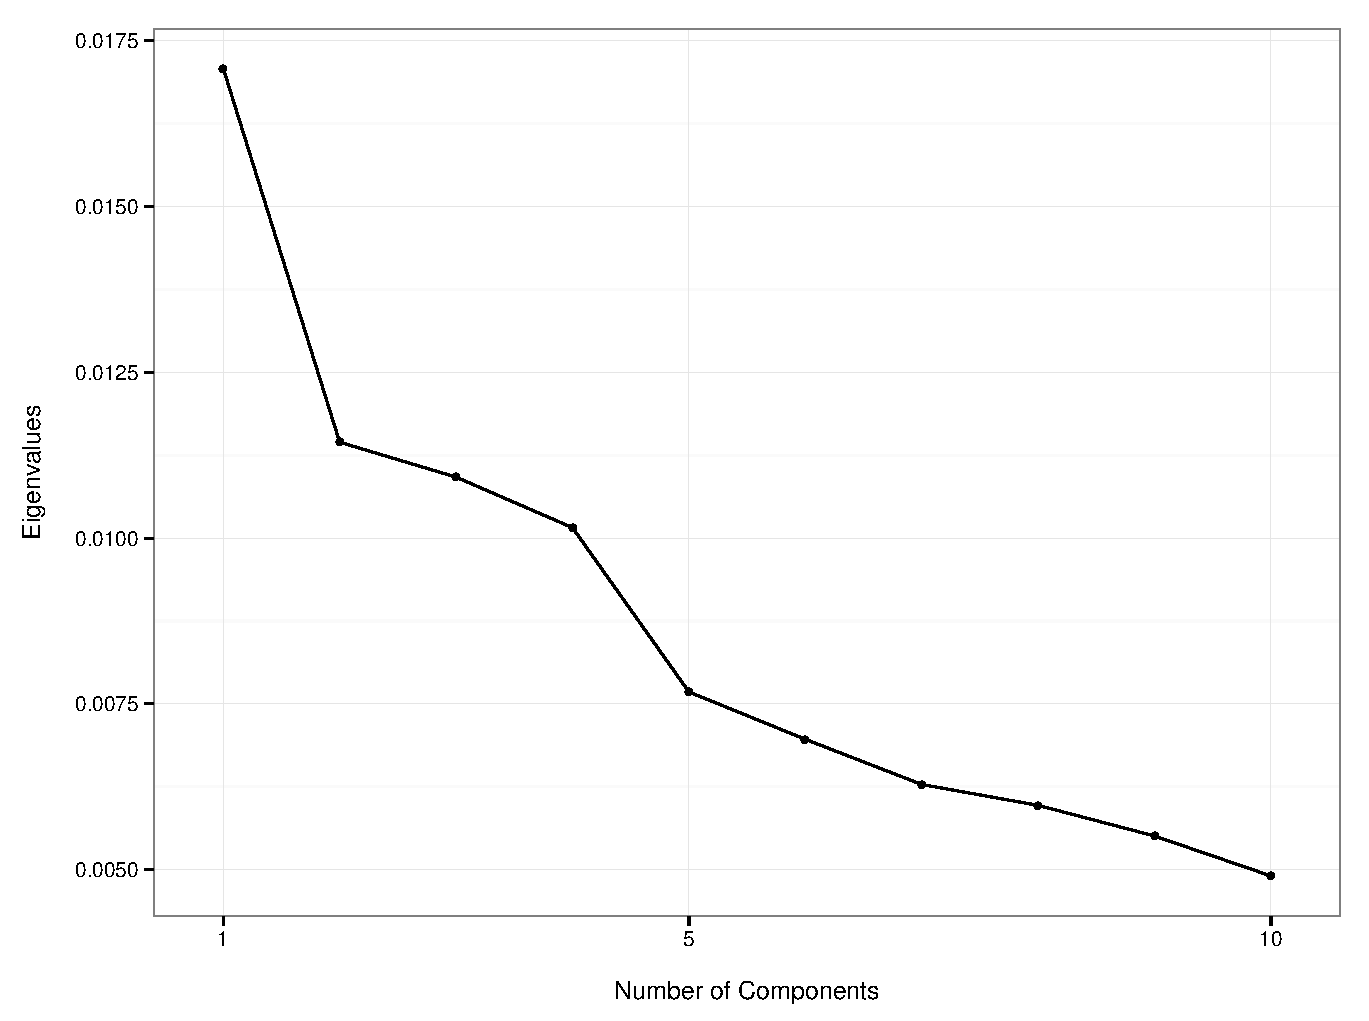
\includegraphics[scale=0.5]{figures/scree_plot.pdf}
    \end{center}
\end{figure}

\section{Validation and Description}\label{results}

The lines in figures \ref{compare_1} and \ref{compare_2} show the results of the kernel PCA analysis--the first principal component--for a wide selection of countries. What does this dimension actually represent? We took a number of approaches to answer this question. First, following \cite{Spirling2012} we used a random forests regression \citep{Breiman2001,jones2015} and stem-component correlations to examine the relationships between word stems from the texts and the Index. Second, we compared the Index to previous indices using an `interocular' test, i.e. comparing plots of the kernel PCA results to our priors on financial market stress informed by previous indices.

\subsection{Random forests and correlations}\label{random-forests}

Spirling \citeyearpar[88-90]{Spirling2012} demonstrated the usefulness of using random forests ``regressions'' to explore what principal components from textual analyses represent. To use this tool to explore our data, we first created a document-term
frequency matrix from the stemmed documents. Effectively this is a \(k \times s\) matrix recording the frequency of each stem in \(\bm{S}\) for each document in \(\bm{K}\). The document-term matrix clearly does not preserve word order. We removed sparse terms, i.e.~kept only stems that were found in 90 percent of the documents. Random forests regressions, as opposed to ordinary least squares regressions, are useful for exploring this data's associations with the estimated principal components because it can handle many variables--in this case 1,116 stems--relative to the number of documents--12,377.

We focus on estimated variable importance from this analysis.\footnote{We conducted the random forests regressions using the \texttt{rfsrc} function from the \textbf{randomForestSRC} R package \citep{randomForestSRCCite}.} Variable importance in this context functions as a measure of how well the frequency of a given stem in a text allows the model to predict the FinStress score for that text. Key results are shown in Figure \ref{rf_importance}.

Unsurprisingly, a number of the stems with the largest variable importance are `bank', `financi', and `loan'. Terms with these stems were used to select the texts. The prevalence of these terms and others that are clearly related to the financial sector, such as `interest', `rate', and `fund', indicate that FinStress is indeed about financial sector conditions and not some other topic. Words relating to the direction of financial conditions are important including, `growth' and `rise'. We can see that words relating to the the macro-political economic environment of finance are also important, including `govern', `imf', and `currentaccount'.

Table \ref{stem_correlations} shows a selection of correlations to help us get a sense of the general directions of the relationships between the stems and the Index not provided by the random forest variable importance estimates. We can see that a number of terms related to debt, financial assistance, the International Monetary Fund, and aid are positively related to FinStress. Suggesting that the positive direction of the scale is in fact capturing periods where policy-makers would perceive higher financial market stress. Words that are generally about positive credit conditions, such as `growth', `surplus', and `boom' are negatively associated with the Index. This suggests that the lower end of the scale indeed indicates more positive financial market conditions. Finally, we can see that adjectives that have seemingly opposite meanings--`stronger' and `weaker'--are both negatively associated with the Index. Such a finding indicates that a kernel PCA approach is useful compared to context-less bag-of-words approaches.

\begin{figure}
    \caption{40 Stems Estimated to be the Most Important for Predicting EIU Perception of Financial Market Stress Index}
    \label{rf_importance}

    \begin{center}
        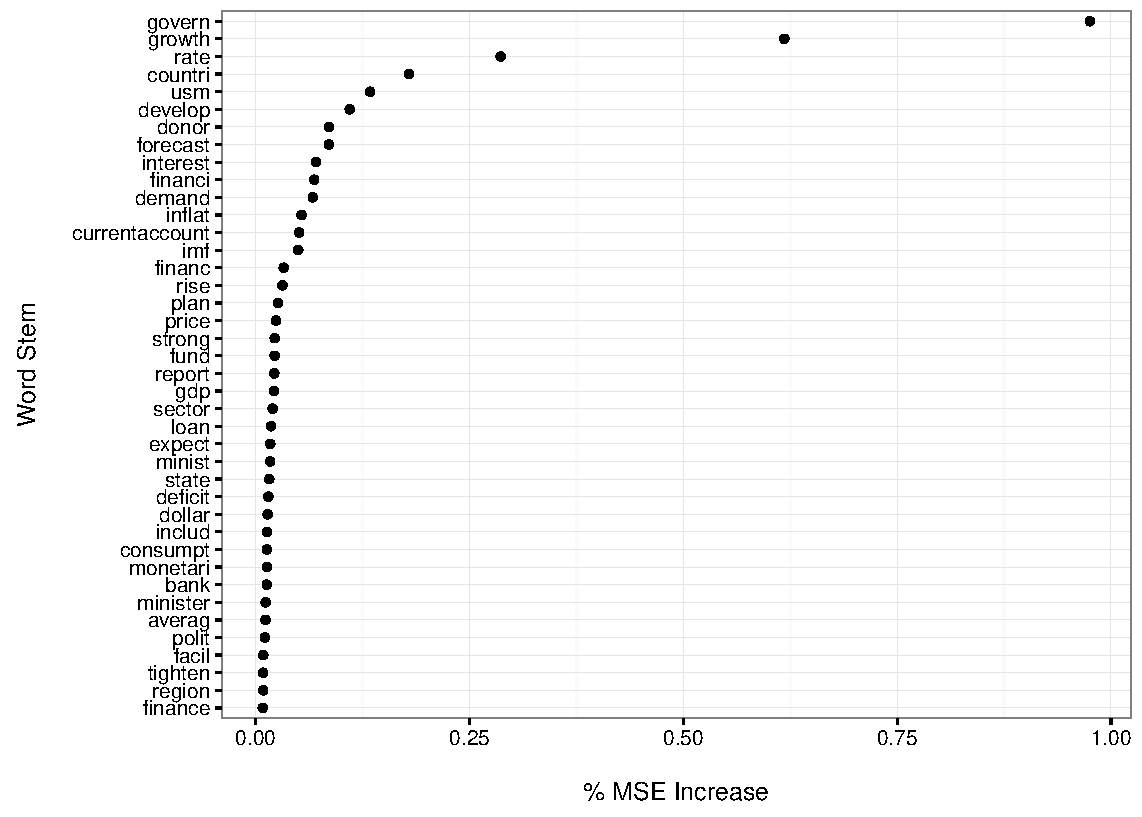
\includegraphics[scale=0.5]{figures/rf_stem_importance.pdf}
    \end{center}

\end{figure}

% latex table generated in R 3.2.1 by xtable 1.7-4 package
% Mon Jun 29 14:16:00 2015
\begin{table}[ht]
\centering
\caption{Selection of Word Stems and Correlations with EPFMS Index} 
\label{stem_correlations}
\begin{tabular}{lr}
  \hline
Stems & Correlations \\ 
  \hline
imf & 0.34 \\ 
  assist & 0.34 \\ 
  aid & 0.28 \\ 
  debt & 0.24 \\ 
  paid & 0.19 \\ 
  strain & 0.09 \\ 
  boom & -0.14 \\ 
  surplus & -0.14 \\ 
  rise & -0.14 \\ 
  weaker & -0.16 \\ 
  stronger & -0.17 \\ 
  growth & -0.28 \\ 
   \hline
\end{tabular}
\end{table}


\subsection{Comparison to other crisis
measures}\label{comparison-to-other-crisis-measures}

How does the Index compare to previous ways of measuring and timing financial market stress and crisis? We directly compare the FinStress Index to the dichotomous measures in \cite{Reinhart2009} and \cite{laeven2013}, as well as Romer and Romer's \citeyearpar{Romer2015} continuous measure.

There are some limitations in comparability simply due to the
different periods of coverage of the different indices. \cite{Romer2015}
in particular largely do not include the most recent crisis in their sample as they did not collect data past 2007. We also had to make a number of transformations and assumptions to be able to directly compare the different data sets. First, the Laeven and Valencia and Reinhart and Rogoff data are recorded at yearly intervals. So, we assumed that the crisis start and end dates they referred to were in the middle of the year, i.e. June.\footnote{In the period covered in figures \ref{compare_1} and \ref{compare_2} this actually improves their fit with events, as many of the 2008 crises became especially apparent after Lehman Brothers collapse in September 2008.} Second, we rescaled Romer and Romer's 16-point scale (in effect 14-points because they do not classify any country-quarter in
their sample as being at the upper two positions on their scale) to be between 0 and 1 using the same method as discussed above for FinStress. Finally, it should be noted that \cite{Romer2015} only cover a selection of OECD countries and \cite{Reinhart2009} only cover 70 countries and their data has been updated least recently.

The solid lines in figures \ref{compare_1} and \ref{compare_2} show the FinStress Index. The dashed lines show Romer and Romer's (rescaled) measure. The shaded boxes show the periods where \cite{laeven2013} and \cite{Reinhart2009} classify there as being a banking crisis.\footnote{We used Table 1 in \cite{Romer2015} to recreate their data set. We downloaded Laeven and Valencia's data from: \url{https://www.imf.org/external/pubs/cat/longres.aspx?sk=26015.0}.
  Accessed May 2015. Reinhart and Rogoff's data was downloaded from:
  \url{http://www.carmenreinhart.com/data/browse-by-topic/topics/7/}.
  Accessed May 2015.} \cite{laeven2013} identify eight ``borderline'' crises in this period, in that the countries almost meet their systemic banking crisis definition because they only used two rather than three policy responses.\footnote{The cases are: France, Hungary, Italy, Portugal, Russia, Slovenia, Sweden, and Switzerland.} Some of these borderline cases are shown in the figures \ref{compare_1} and \ref{compare_2}.

In many cases--conditional on the coverage of each data series--the indices do substantively overlap. Comparisons with \cite{Romer2015} are limited, but we can see that, where comparable time series are available, FinStress and their index are sometimes roughly similar. In particular, both indices increase in the US from early 2007. A notable difference is how Romer and Romer classify Japan as being without stress from mid-2005, while FinStress remains relatively high, especially compared to many other economically developed countries at that time. While both indices classify Iceland as being under stress in the late 2000s, the timing is different. Romer and Romer classify Iceland as in stress\footnote{They classify Iceland as being in a ``minor crisis'' in the second half of 2006 and a ``credit  disruption'' in the first half of 2007.} in 2006-2007. This is earlier than not only a marked increase in the FinStress Index, but also Reinhart and Rogoff and Laeven and Valencia's timing.

\cite{Reinhart2009} sometimes start dating a crisis before \cite{laeven2013}--particularly in Iceland and Ireland. This could reflect the slightly different definitions that they use. As summarised in Table \ref{comp_table}, \cite{Reinhart2009} date crises from when bank runs occur. \cite{laeven2013} begin the crisis clock when there is not only significant financial system distress, but also when the government follows the distress with a policy response.

One useful characteristic of FinStress is that we can use it to follow the progression of crisis intensity over time. \cite[227]{laeven2013} comment that part of the problem with dating financial crises is that each develops differently:

\begin{quote}
    Some crises evolve gradually, gaining speed as the ripple effects from a seemingly small shock propagate forward in time \ldots other episodes happen more abruptly and are often the result of sudden stops.
\end{quote}

\noindent FinStress' real-time and relatively granular nature allows us to distinguish these types of crises. For example, we can see in Figure \ref{compare_2} that financial market difficulties in the United States crisis built over a long period of time, with a few spikes during notable banking difficulties, e.g. Lehman Brothers collapse. Conversely, countries such as Germany, Hungary, and Iceland clearly have much more sudden periods of perceived financial distress. Using an binary definition of crises would no allow us to capture these trajectories.

We can use the EPMFS to identify periods where financial market
conditions were perceived to be worsening, though for whatever reason these perceptions changed before other measures would record a financial crisis. Australia, Brazil, and the Czech Republic, among others, in about late-2008/2009 are notable examples. They all see clear spikes in perceptions of stress shortly after Lehman Brothers collapsed in the US. Fairly quickly thereafter, their EPMFS scores returned to previous levels. Laeven and Valencia and Reinhart and Rogoff do not record these episodes as crises. The perceived stress likely experienced by policy-makers at this time would therefore be excluded from political science work using binary measures of crisis.

The advantages of FinStress are also apparent for timing the end of heightened financial market distress. This is a particularly difficult issue for the established binary indicators. Crisis onset is typically well defined by these measures, but they rarely have a clear or non-ad hoc way of determining when a crisis has ended. Though, we are limited by the time period coverage of the EIU texts we have at our disposal, it is clear that some countries, notably the Netherlands, Switzerland, the United Kingdom and the United States, were perceived to be having improved financial market conditions from about 2010. Other countries, particularly Eurozone countries in Western and Southern Europe plateaued at a high level through the end of 2011. Laeven and Valencia's measure simply describes these entire periods as a crisis. Not only does the EPMFS allow us to more accurately date when conditions were seen to have improved, but it also allows us to study the trajectory of these improvements.

Overall, the similarities between FinStress scores and other measures of crises suggests that FinStress Index does capture financial market stress. In particular, higher FinStress values are indicative of higher levels of perceived financial market stress. At the same time, the differences between the measures indicate that FinStress sheds unique light on processes not captured well by previous indices. One major difference that we will now look at in more detail is how having a continuous indicator allows us to consider how levels perceived financial market stress differ between developed and developing countries.

\begin{figure}
    \caption{Comparing Perceptions of Financial Market Conditions to \cite{laeven2013} and \cite{Reinhart2009} (1)}
    \label{compare_1}
    \begin{center}
        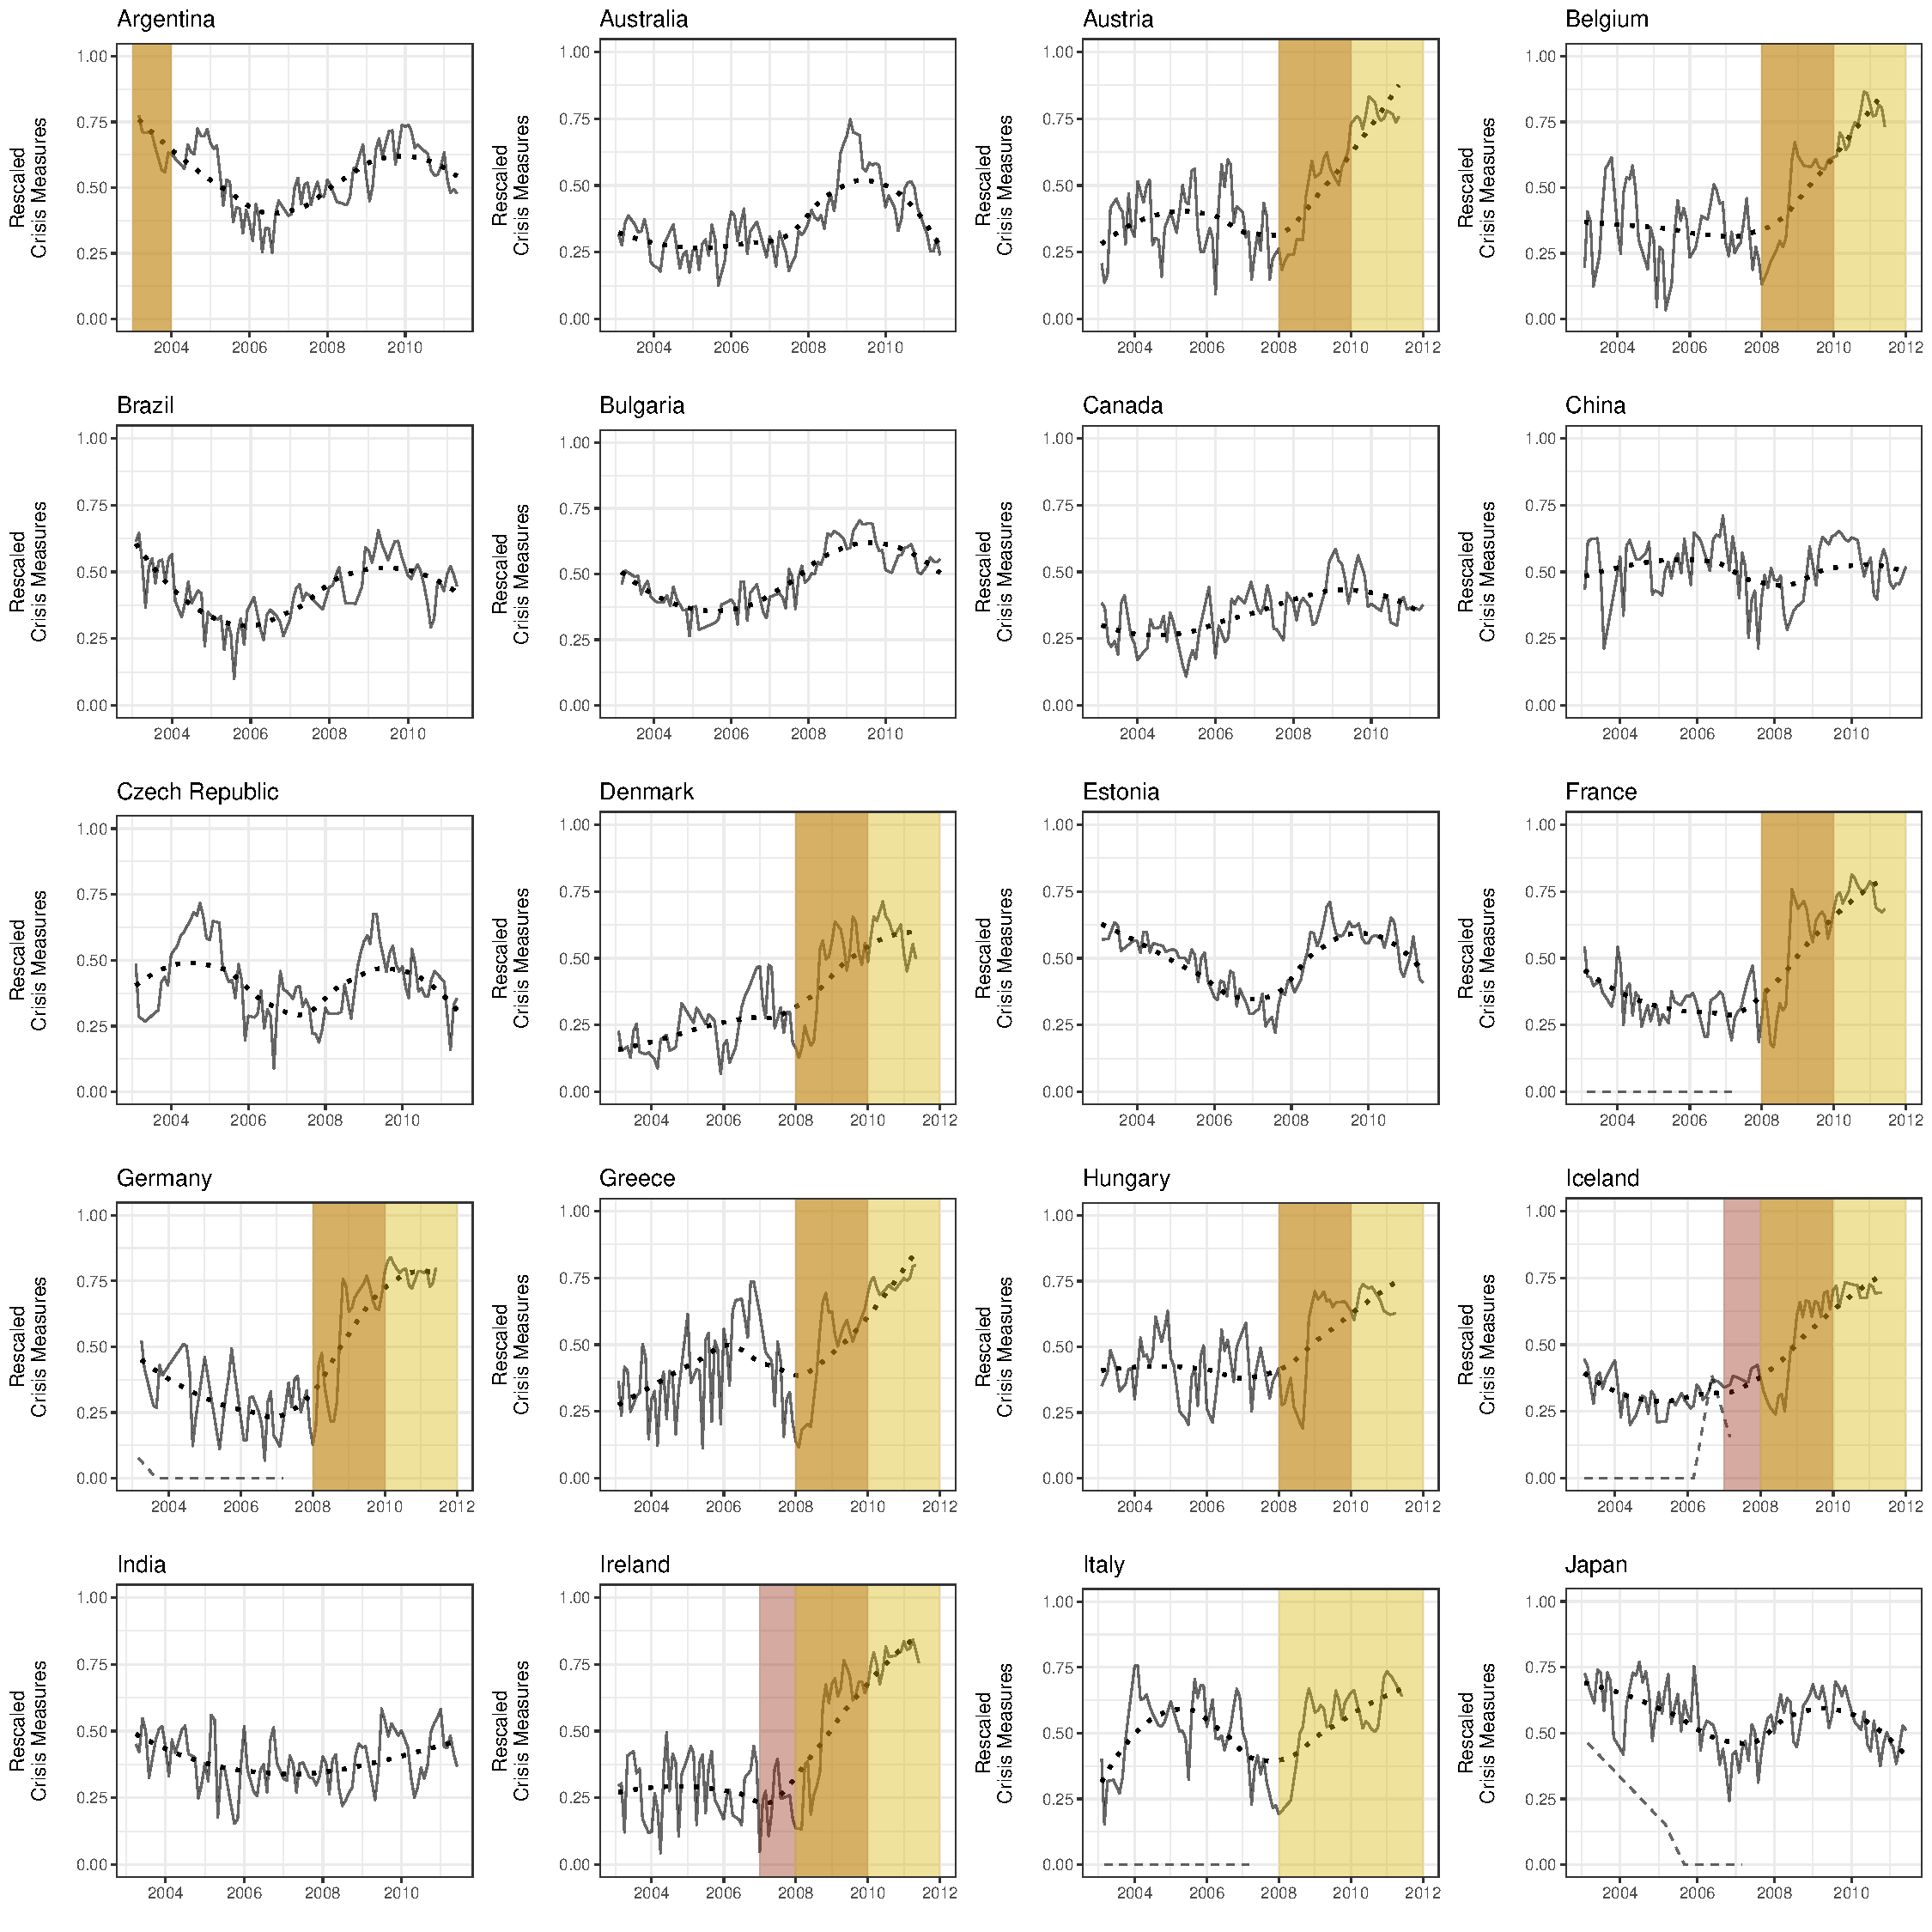
\includegraphics[scale=0.4]{figures/compare_to_lv_rr.pdf}
    \end{center}

    {\tiny{Solid lines show the (rescaled) EIU Perceptions of Financial Market Stress indicator. Dotted lines represent a loess smooth of these series. \\

    Yellow shaded areas indicate periods that \cite{laeven2013} classify as systemic banking crises. Note that crises are automatically terminated at the end of 2011 due to the series not extending beyond this point, not necessarily because the crisis finished. \\

    Red shaded areas indicate periods that \cite{Reinhart2009} classify as banking crises. Note that crises are automatically terminated at the end of 2009 due to the series not extending beyond this point, not necessarily because the crisis finished. \\

    Orange areas indicate periods where a crisis is recorded for both measures.}}
\end{figure}

\begin{figure}
    \caption{Comparing Perceptions of Financial Market Conditions to \cite{laeven2013} and \cite{Reinhart2009} (2)}
    \label{compare_2}
    \begin{center}
        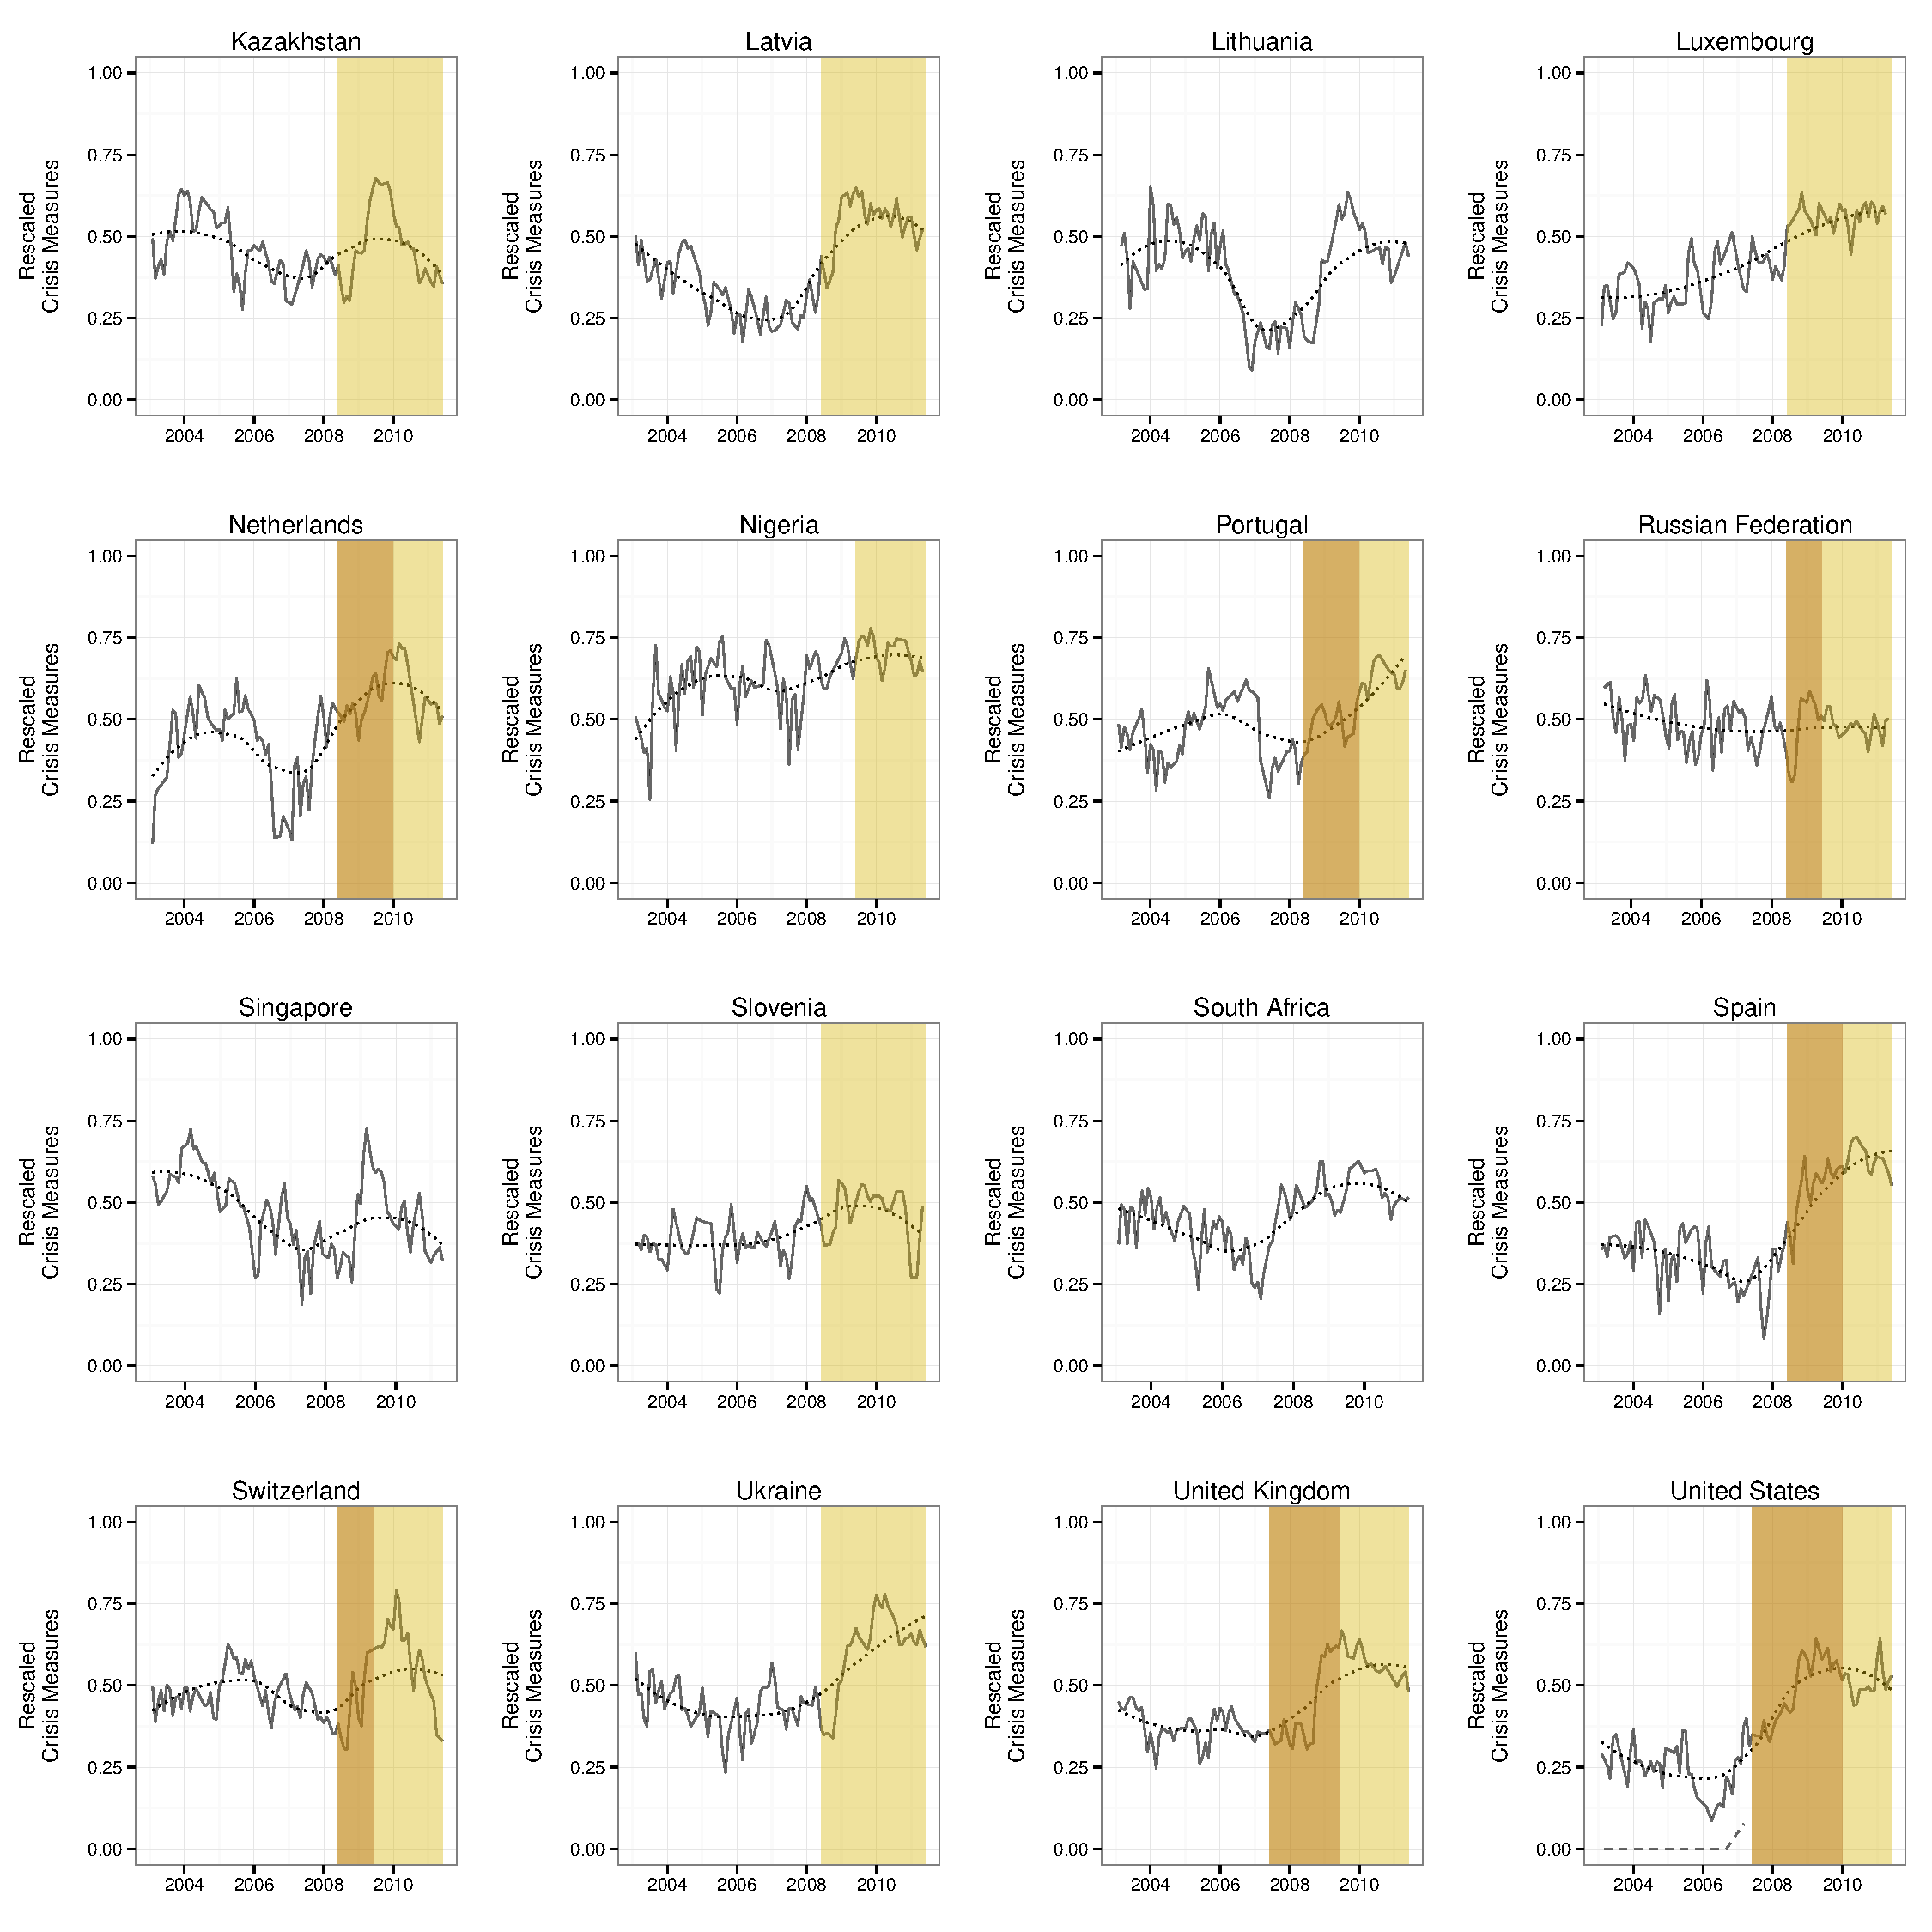
\includegraphics[scale=0.4]{figures/compare_to_lv_rr_2.pdf}
    \end{center}

    {\tiny{Solid lines show the (rescaled) EIU Perceptions of Financial Market Stress indicator. Dotted lines represent a loess smooth of these series. \\

    Dashed lines show Romer and Romer's \citeyearpar{Romer2015} index rescaled. \\

    Yellow shaded areas indicate periods that \cite{laeven2013} classify as systemic banking crises. Note that crises are automatically terminated at the end of 2011 due to the series not extending beyond this point, not necessarily because the crisis finished. \\

    Red shaded areas indicate periods that \cite{Reinhart2009} classify as banking crises. Note that crises are automatically terminated at the end of 2009 due to the series not extending beyond this point, not necessarily because the crisis finished. \\

    Orange areas indicate periods where a crisis is recorded for both measures.}}
\end{figure}

\clearpage

\subsection{Developed vs.~developing
countries}\label{developed-vs.developing-countries}

Examining the Index, it is clear that there is a difference in the level of perceived financial market stress in developed and developing countries. Developing countries often have higher FinStress scores. The mean score in middle and low income countries (as classified by the World Bank) is 0.53 in 2005, a relatively placid year. While many developed countries only reach this level during financial crises (see Figure \ref{comp_dev_developing}).\footnote{The 2005 mean for high income countries is 0.44} The distribution of FinStress scores in these two groups of countries is significantly different in the expected direction in the sample using one-sided Kolmogorov-Smirnov tests.\footnote{We ran the tests using the \texttt{ks.test} function from base R.}

Developing countries often lack strong financial institutions and systems, so we should expect them to face generally tighter credit market conditions than developed countries. As a consequence, they are more likely to be receiving assistance from multilateral parties, such as the IMF. This is all to say that financial markets are generally more stressed in developing as opposed to developed countries.

This observation leads to important refinements to our understanding of how the Index should be interpreted and how it should be used in empirical work. First, the Index measures banking market conditions, but not `crisis' directly. Instead, perceived crisis is likely the result of an interaction between financial market stress and the importance of financial markets for sustaining a country's economy. Though policy-makers in developing economies face generally tight credit market conditions, these persistent conditions likely do not threaten the wider \emph{status quo} economy. As such, we would not expect significant policy responses to address financial market stress in these places. Conversely, tightening credit market conditions in a developed, financialised economy would likely have large negative changes to the wider economy. So, we would expect politicians in these countries to respond to worsening credit market conditions. Previous measures of financial market distress and crises would not be able to explore this possible interaction.

\begin{figure}
    \caption{Comparison of Mean FinStress Scores in High vs. Low and Medium Income Countries}
    \label{comp_dev_developing}

    \begin{center}
        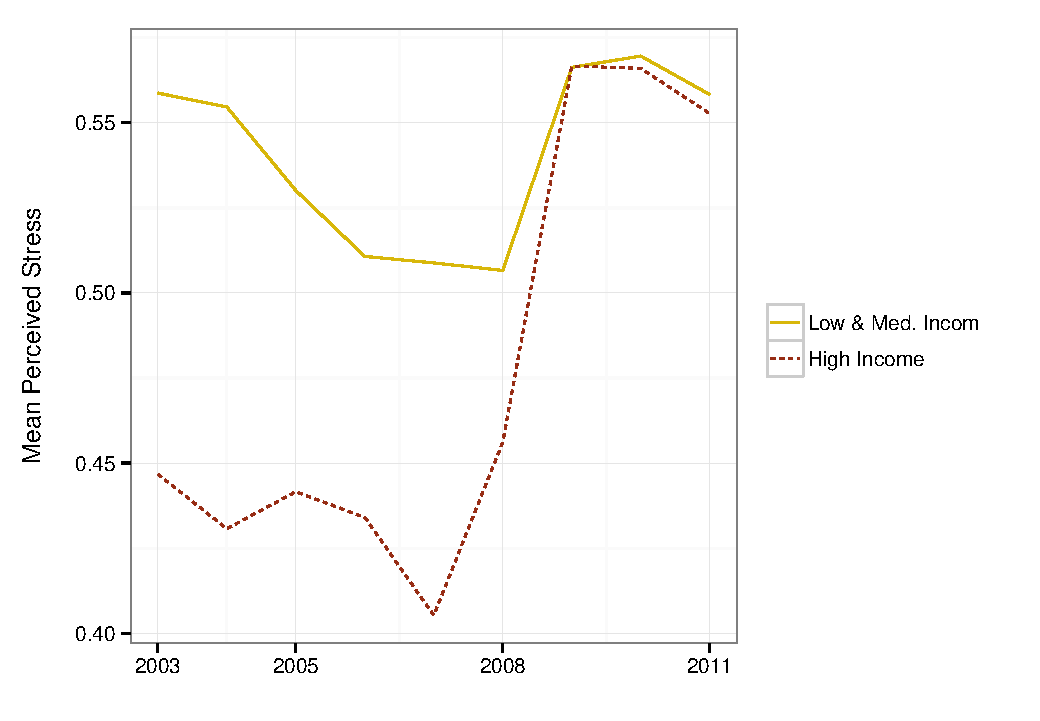
\includegraphics[scale=0.45]{figures/dev_vs_devoloping.pdf}
    \end{center}
\end{figure}

\subsection{Comparison to accounting measures of banking system fragility}

How does FinStress compare to the widely used Z-Score measure of banking system fragility? Though the two quantities measure different phenomenon--perceptions for the former and bank accounting relationships for the latter--potentially both provide indications of stress. We might expect them to be related to one another, either being positively correlated and/or one acting as a leading indicator of the other.

To explore these possible associations, we compare FinStress to the Bank Z-Score measure compiled from Bankscope data in the World Bank's Global Financial Development Database (GFDD) project \citep{worldbank2013}.\footnote{Indicator ID: GFDD.SI.01. Accessed June 2015.} The measure is interpretable as the inverse of the upper bound of the probability of the banking system's insolvency.\footnote{Formally: $\frac{\mathrm{ROA}_{t} + \frac{\mathrm{equity}_{t}}{\mathrm{assets}_{t}}}{\sigma_{\mathrm{ROA}}}$. $\mathrm{ROA}$ is return on equity. $\sigma_{\mathrm{ROA}}$ is presumably for the entire period for which data is available, though the World Bank's documentation does not explicitly specify this. It is common in other work for the $\sigma_{\mathrm{ROA}}$ to be based on a three year rolling window \cite[225]{beck2013bank}. All quantities are country aggregates.} Figure~\ref{z_score} shows a comparison of the two measures for selected countries. Note that to ease visual comparability we rescaled the Z-Scores to be within zero and one as before, and reversed the scale so that larger values indicate a higher probability of banking system insolvency.\footnote{It is common to log-transform the Z-Scores \cite[225]{beck2013bank}. However, it is unclear how previous work has done this as there are negative values in the Z-score that would create undefined values when logged.} Finally, we converted FinStress to yearly averages for comparability.

There does not appear to be a relationship between Z-Scores and FinStress Index. The rescaled Z-Score is positively correlated with FinStress, but this is not significant at the 10\% level. Interestingly, the World Bank's Z-Scores do not vary significantly within countries over time, especially compared to  FinStress. There is little difference between Z-Scores for countries during periods of heightened financial stress (however measured) and more stable times. Thus Z-Scores, at least those provided by the World Bank, are not a useful indicator of financial crisis states. Z-Scores do not appear to predict perceptions of financial market stress. In a simple partial correction linear regression that had FinStress as the dependent variable and included lagged FinStress, lagged Z-Scores, and country fixed-effects, Z-Scores were not statistically significantly associated with perceptions of financial market stress (see the Online Appendix).

It is beyond the scope of our article to determine why the Z-Score--at least the version available through the World Bank's GFDD--is a sub-optimal cross-time measure of financial market stress. However, the measure's peculiar characteristics are important to note for future researchers: the indicator has weak time-variance, it does not distinguish between periods of significant known financial market stress and less stressful times, and it does not help us predict perceived financial market stress.

\begin{figure}

    \caption{Annual Mean FinStress Compared to Country-level Z-Scores (rescaled)}
    \label{z_score}

    \begin{center}
        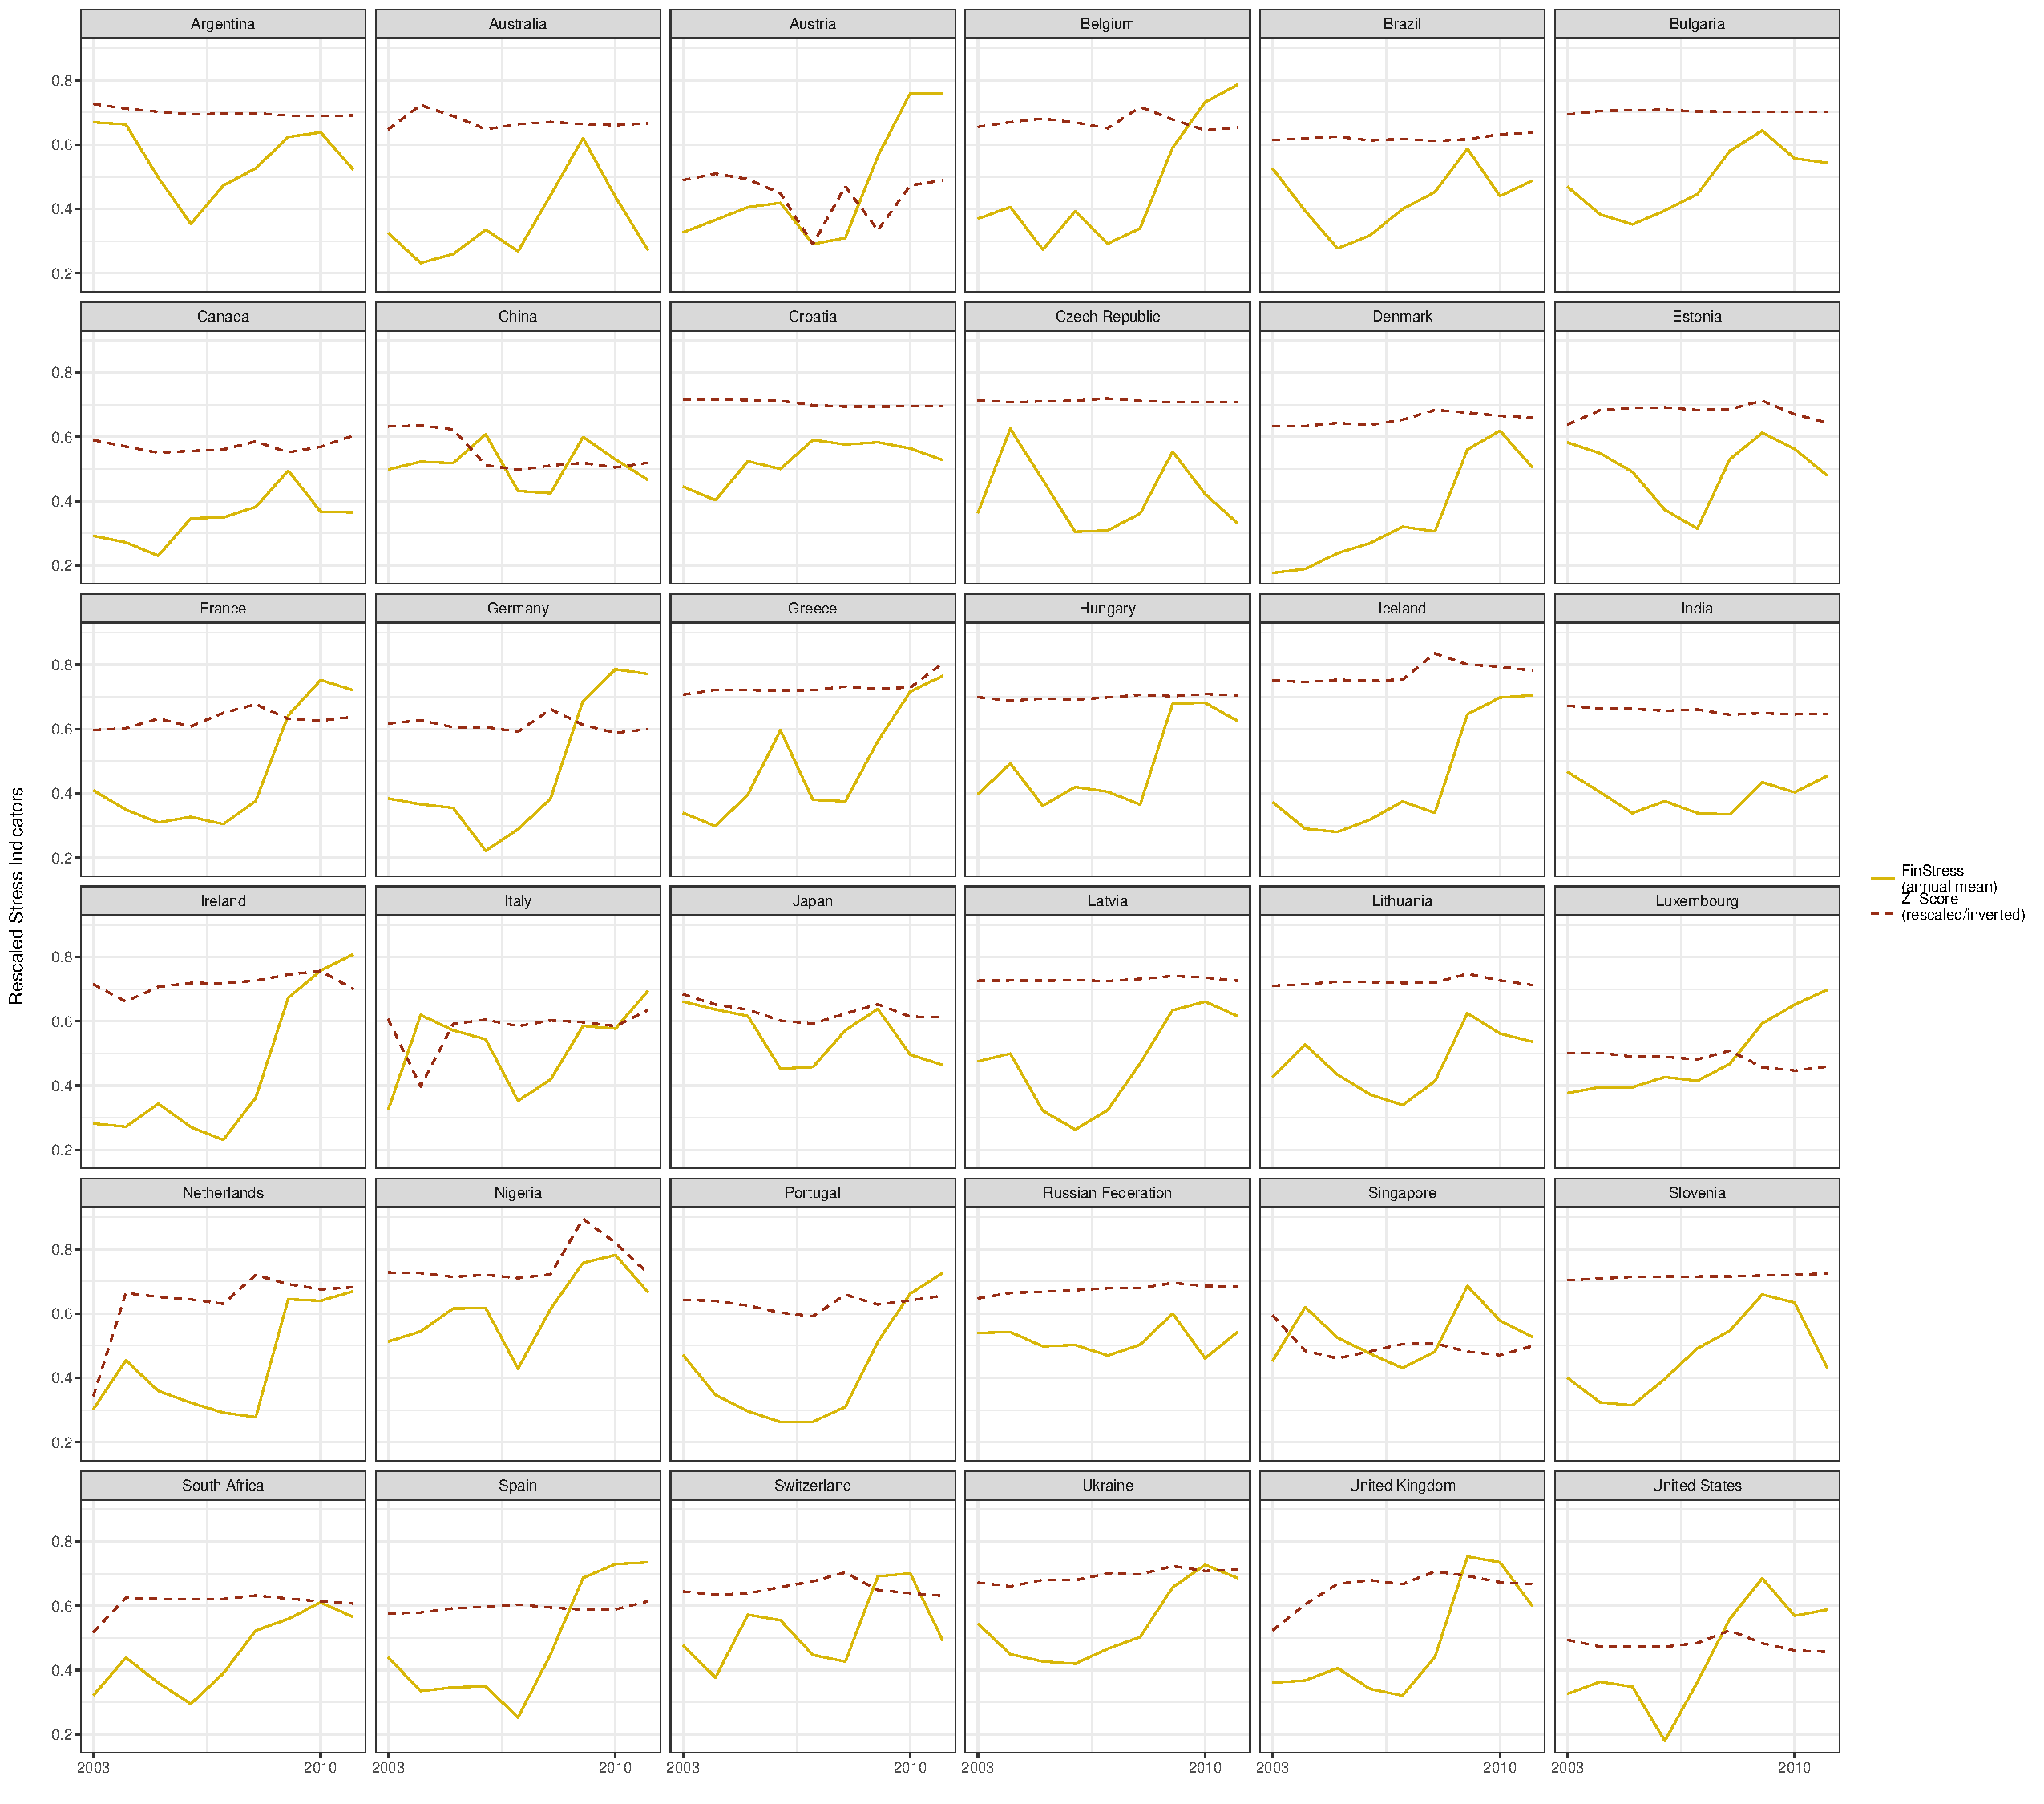
\includegraphics[scale=0.4]{figures/compare_to_z-score.pdf}
    \end{center}

\end{figure}

\section{Summarising FinStress changes}

So far we have largely examined FinStress \emph{levels}. Now we turn to examining  FinStress level \emph{changes}. To do this we use a nonparametric drift-diffusion-jump model \citep[DDJ,][]{Carpenter2011,Dakos2012}. This approach allows us to draw general conclusions about how perceptions of financial market stress change in more demanding and less demanding times.

DDJ models allow us to approximate processes of change in a time series without needing to make explicit assumptions about the underlying process that creates these changes.\footnote{It should be stressed that unlike in other applications of DDJ models, such as in ecology and related work in finance \citep{Kou2008}, that use them to predict future states. We exclusively use this statistical approach to summarise changes and elucidate patterns in observed data, rather than predict future events.} Drift is a measure of the local rate of change. Diffusion is small changes that happen at each time increment. Jumps are larger shocks that occur intermittently and are uncorrelated in time. The approach we take to estimating the DDJ model is from \cite{Carpenter2011}.\footnote{The model approximates the unknown process generating FinStress scores: $dx_{t} = f(x_{t},\;\theta_{t})dt + g(x_{t},\;\theta_{t})dw + dJ_{t}$. $dx_{t}$ is the change in the FinStress score $x$ for a country at time $t$. $\theta_{t}$ is a critical transition parameter. The drift function is given by $f(x_{t}\theta_{t})dt$. The diffusion function is given by $g(x_{t}\theta_{t})dw$. $J$ is a jump process. Please see Dakos et al. \citeyearpar[7]{Dakos2012} for further details. We estimated the model using the \texttt{ddjnonparam\_ews} function from the \textbf{earlywarnings} R package \citep{earlywarnings2013}. Note that we estimated the parameters for each country's time series separately.}

In the abstract, we would perhaps expect that jumps would be more common in countries' FinStress scores during crisis periods, because there would be large moves in the Index. To test this we first graphically compared the distributions of jump and diffusion parameters across what Laeven and Valencia\footnote{Despite the previously discussed shortcomings, they are the most recently updated and comprehensive binary measure of crises.} classify as crisis and non-crisis periods. Figure \ref{comp_jump_diff} shows these densities. We have also included a measure of total variance, which is a summary of both jump and diffusion parameters.

\begin{figure}
    \caption{Diffusion, Jump, and Total Variance Estimate Distributions Across Crisis and Non-Crisis Periods from \cite{laeven2013}}
    \label{comp_jump_diff}
    \begin{center}
        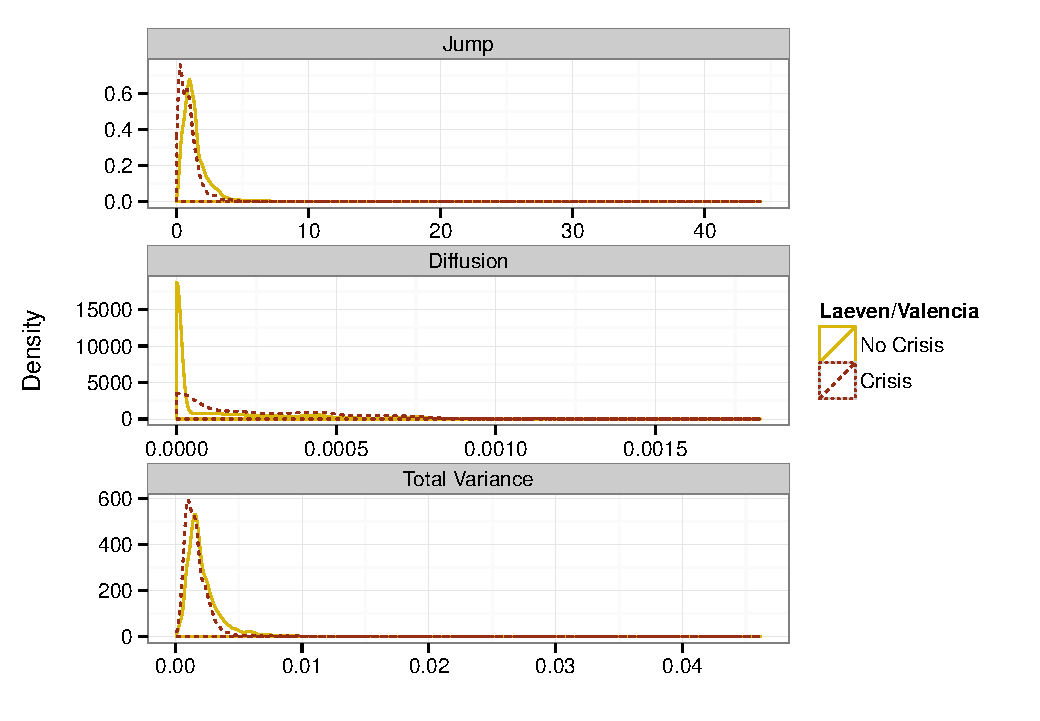
\includegraphics[scale=0.7]{figures/compare_jump_diffusion_basic.pdf}
    \end{center}
\end{figure}

We can see that the distribution of estimated jump parameters in `non-crisis' periods is shifted upward from the distribution of jump parameters in `crisis' periods. Conversely, the distribution of diffusion parameters in crisis periods is shifted upward from non-crisis periods. Finally, the distribution of total variance in crisis periods is lower than non-crisis periods. We found these distributions to be statistically significantly different in the described direction at all conventional levels using one-sided Kolmogorov–Smirnov tests.\footnote{Again, we ran the tests using the \texttt{ks.test} function from base R.}

This is an counter-intuitive result considering our prior expectations. How can we make sense of it? It is useful to refer back to figures \ref{compare_1} and \ref{compare_2}. Notice that some of the periods that are classified across measures as a crisis do indeed begin with a jump. Iceland and Ireland in 2008 are particularly illustrative of this. What happens after the jump is interesting. Before crisis periods there are sometimes large swings in both positive and negative directions. In crisis periods there are a few periods of large positive changes followed by many smaller, often positive, FinStress changes at a high level.

In non-crisis times there may effectively be more noise in economic events about the underlying level of stress, causing relatively large positive \emph{and} negative swings in perceptions of financial market conditions, e.g. is the failure of one bank indicative of wider problems to come or is it a local event caused by, for example, ineffective management at that particular bank? When crises occur, the information used to create perceptions of financial market stress is clearer. Think for example of Lehman Brother's collapse and the continually bad news that followed. During a crisis, initial shocks are followed by additional bad news that reinforces perceptions of heightened stress. During non-crisis times, a possible shock could be relatively quickly followed by good news, returning perceptions of stress to a lower level.

Not all crises are the same. Many of the crises in the period for which we have data have been protracted. In some cases, however, crises came quickly and left almost as quickly. Kazakhstan is a notable example. In late 2009 there was a prominent spike in perceptions of financial market stress. Within a few months, the country's FinStress score returned to almost its previous trend level. There could be a number of reasons for this type of trajectory, including effective policy responses that quell stress and market actors having inaccurate information about financial conditions that takes a longer than usual period to be corrected.

\section{Application}\label{application}

A clear use for the FinStress Index is as a right-hand covariate in regression analyses where the dependent variable is, for example, a particular policy choice or government failure time. The Index could also be used as a dependent variable such that we could examine how, for example, government partisanship or electoral competitiveness affects perceptions of financial stability. In this section we show how FinStress can be useful for examining political budget cycles during periods of financial market stress.\footnote{This section is based on work primarily developed in \cite{gandrudHallerbergPBC}.}

\subsection{Problems measuring fiscal responses to financial crises}

Measuring the fiscal costs of financial crises is notoriously difficult \citep[see][]{reinhartRogoff2011}. \cite{GandrudHallerberg2015} catalogue many issues with perhaps the most comprehensive data set of fiscal costs: Laeven and Valencia \citeyearpar[and their predecessors]{laeven2013}. There are many different avenues to assist ailing financial institutions, many of which, like guarantees and liquidity assistance, may not involve direct expenditures that are easily attributable to a specific policy choice. Accounting rules differ across time and place \citep{gandrudHallerbergWEP} meaning that a cost in one context may be ``hidden debt'' \citep{reinhartRogoff2011} in another.

We should also expect costs to vary according to crisis severity, not just policy-makers choices. Politicians will, on average, respond more forcefully to resolve what they perceive to be more severe financial market stress to achieve the same level of financial stability. We need to be able to account for how severe politicians believe their crises to be.

When costs are realised may be endogenous to political conditions. Politicians have some control over the timing of when financial crisis costs are exposed. For example, the United Kingdom's Chancellor of the Exchequer George Osborne announced on 10 June 2015 that the government would begin selling its stake in the Royal Bank of Scotland (RBS)--a bank that had been nationalised during the 2008 crash. The sale would likely be at a substantial loss.\footnote{See \url{http://www.theguardian.com/business/2015/jun/10/george-osborne-signals-rbs-sell-off-at-mansion-house-speech}. Accessed June 2015.} The sale announcement was made approximately a month after the United Kingdom's general election in which George Osborne's Conservative Party was re-elected and won a parliamentary majority. In consequence, if not design, the realisation of these losses from assisting RBS was deferred until after the election, when the government had secured another five year period in power before they needed to return to voters.

This event raises an interesting question: what political factors influence \emph{when} politicians decide to make the costs of a financial crisis public? To the extent that they can control cost realisation timing, do they, like George Osborne, choose to reveal costs when they are sitting on the safe side of an election? We can use FinStress to help us answer these questions.

\subsection{Estimating `off-trend' financial crisis debt}

To answer these questions we first need to consider what aspect of governments' fiscal positions voters, and so office-seeking politicians, are primarily concerned about. \cite{gandrudHallerbergWEP} argue that voters likely pay the most attention to gross debt increases. Taxpaying voters are wary of debt increases as they might lead to tax increases. Voters who benefit more from government spending are also concerned about debt increases as these might lead to spending cuts. We would therefore expect office-seeking politicians to try to shift gross debt increases until after elections, when they are under the least threat of being removed from office by displeased voters.

It is likely that governments can only defer realising the costs of responding to financial crises until after elections on the margins. Voters are not only worried about debt increases. They are also concerned with general economic well-being, and therefore want governments to restore financial market stability when markets become unstable \citep{Rosas2009}. Stabilising financial markets involves policies, such as guaranteeing deposits or providing liquidity assistance to banks such that most of the costs will likely increase the debt in a way that is not deferrable by the government. We would expect that on average debts will be higher when there is more financial market stress. Additionally, we would expect debts to be higher when the economy is doing worse generally, regardless of whether or not this is caused by financial or other crises. Especially in advanced democracies, previous policy decisions have created automatic stabilisers, like unemployment insurance, that are more costly during crises.

\begin{table}
    \caption{Estimating Off-Trend Central Government Debt in Response to Financial Market Stress}
    \label{residuals}
        \begin{center}
            
% Table created by stargazer v.5.2 by Marek Hlavac, Harvard University. E-mail: hlavac at fas.harvard.edu
% Date and time: Wed, Jul 29, 2015 - 11:09:17
\begin{tabular}{@{\extracolsep{5pt}}lc} 
\\[-1.8ex]\hline 
\hline \\[-1.8ex] 
 & \multicolumn{1}{c}{\textit{Dependent variable:}} \\ 
\cline{2-2} 
\\[-1.8ex] & Central Gov. Debt \% GDP (2005 GDP rebased) \\ 
\hline \\[-1.8ex] 
 Debt$_{t-1}$ & 0.902$^{***}$ \\ 
  & (0.045) \\ 
  & \\ 
 FinStress & 19.360$^{***}$ \\ 
  & (4.773) \\ 
  & \\ 
 Output Gap & $-$0.055 \\ 
  & (0.136) \\ 
  & \\ 
 Constant & $-$1.551 \\ 
  & (3.600) \\ 
  & \\ 
\hline \\[-1.8ex] 
country fixed effects & Yes \\ 
\hline \\[-1.8ex] 
Observations & 264 \\ 
R$^{2}$ & 0.974 \\ 
Adjusted R$^{2}$ & 0.970 \\ 
Residual Std. Error & 5.706 \\ 
F Statistic & 257.595$^{***}$ \\ 
\hline 
\hline \\[-1.8ex] 
\textit{Note:}  & \multicolumn{1}{r}{$^{*}$p$<$0.1; $^{**}$p$<$0.05; $^{***}$p$<$0.01} \\ 
 & \multicolumn{1}{r}{Standard errors in parentheses.} \\ 
\end{tabular} 

        \end{center}
\end{table}

To estimate marginal `off-trend' government debt changes in response to financial crises we ran a partial correction panel regression with central government debt as a percentage of GDP as the dependent variable. This variable is from the World Bank's Development Indicators.\footnote{\url{http://data.worldbank.org/data-catalog/world-development-indicators}. Accessed June 2015. It was originally recorded as a percentage of the same year GDP. To strip out GDP changes--we are only interested in changes to the numerator not the denominator--, we rebased the variable in terms of each countries' 2005 GDP. The GDP variable was from the OECD.} The results are shown in Table \ref{residuals}. The model includes lagged central government debt as a percentage of GDP to control for serial autocorrelation and countries' output gaps to control for general economic declines. The model also includes country fixed effects. The output gap is from the OECD\footnote{Data was accessed through \url{https://data.oecd.org/} in June 2015.} and as such our sample is constricted to OECD members.

As expected, we can see that perceptions of financial market stress are very strongly positively associated with higher gross central government debt. Predictions from this model can be considered as the average or `trend' central government debt at various levels of perceived financial market stress. Residuals from the model can be thought of as how far `off-trend' a country-year is given a particular level of perceived stress.

\begin{table}
    \caption{Estimating Marginal Changes in Off-Trend Central Government Debt in Response to Crises}
    \label{results_elect}
    \begin{center}
        
% Table created by stargazer v.5.1 by Marek Hlavac, Harvard University. E-mail: hlavac at fas.harvard.edu
% Date and time: Tue, Jul 14, 2015 - 12:26:57
\begingroup 
\tiny 
\begin{tabular}{@{\extracolsep{5pt}}lcccccc} 
\\[-1.8ex]\hline 
\hline \\[-1.8ex] 
 & \multicolumn{6}{c}{\textit{Dependent variable:}} \\ 
\cline{2-7} 
\\[-1.8ex] & \multicolumn{6}{c}{$\Delta$ Off-Trend Debt} \\ 
\\[-1.8ex] & (1) & (2) & (3) & (4) & (5) & (6)\\ 
\hline \\[-1.8ex] 
 $\Delta$ Off-Trend Debt$_{t-1}$ & $-$0.409$^{***}$ & $-$0.393$^{***}$ & $-$0.350$^{***}$ & $-$0.393$^{***}$ & $-$0.182$^{*}$ & $-$0.510$^{***}$ \\ 
  & (0.089) & (0.088) & (0.084) & (0.089) & (0.093) & (0.116) \\ 
  & & & & & & \\ 
 $\Delta$ Off-Trend Spend &  &  &  &  & 1.187$^{***}$ &  \\ 
  &  &  &  &  & (0.257) &  \\ 
  & & & & & & \\ 
 $\Delta$ Off-Trend Spend$_{t-1}$ &  &  &  &  &  & 0.892$^{**}$ \\ 
  &  &  &  &  &  & (0.388) \\ 
  & & & & & & \\ 
 Post-Election Yr. & 2.585$^{*}$ & 6.150$^{**}$ & 5.546$^{**}$ & 6.182$^{**}$ & 5.449$^{**}$ & 5.161$^{**}$ \\ 
  & (1.463) & (2.377) & (2.267) & (2.393) & (2.387) & (2.558) \\ 
  & & & & & & \\ 
 Loss Prob. & $-$2.428 & 1.706 & 3.962 & 2.046 & 6.343$^{*}$ & 4.026 \\ 
  & (5.710) & (6.052) & (3.485) & (6.135) & (3.781) & (4.027) \\ 
  & & & & & & \\ 
 Econ Ideology &  &  &  & $-$0.887 & $-$0.702 & $-$0.730 \\ 
  &  &  &  & (1.012) & (0.747) & (0.802) \\ 
  & & & & & & \\ 
 Political Constraints &  &  &  & $-$0.596 & $-$0.289 & $-$0.930 \\ 
  &  &  &  & (9.019) & (5.802) & (6.219) \\ 
  & & & & & & \\ 
 Fixed FX &  &  &  & 0.124 & $-$1.373 & $-$0.972 \\ 
  &  &  &  & (4.126) & (1.521) & (1.627) \\ 
  & & & & & & \\ 
 Post-Election Yr. * Loss Prob. &  & $-$12.599$^{*}$ & $-$11.413$^{*}$ & $-$12.778$^{*}$ & $-$12.337$^{*}$ & $-$10.467 \\ 
  &  & (6.667) & (6.319) & (6.784) & (6.962) & (7.472) \\ 
  & & & & & & \\ 
 Constant & 0.304 & $-$0.738 & $-$1.781 & 1.461 & $-$0.241 & 0.592 \\ 
  & (3.578) & (3.578) & (1.186) & (6.049) & (3.712) & (3.983) \\ 
  & & & & & & \\ 
\hline \\[-1.8ex] 
country fixed effects & Yes & Yes & No & Yes & No & No \\ 
\hline \\[-1.8ex] 
Observations & 132 & 132 & 132 & 132 & 113 & 113 \\ 
R$^{2}$ & 0.239 & 0.264 & 0.177 & 0.270 & 0.318 & 0.218 \\ 
Adjusted R$^{2}$ & 0.069 & 0.091 & 0.151 & 0.080 & 0.266 & 0.158 \\ 
Residual Std. Error & 7.490 & 7.402 & 7.151 & 7.445 & 7.046 & 7.547 \\ 
F Statistic & 1.403 & 1.522$^{*}$ & 6.834$^{***}$ & 1.422 & 6.070$^{***}$ & 3.623$^{***}$ \\ 
\hline 
\hline \\[-1.8ex] 
\textit{Note:}  & \multicolumn{6}{r}{$^{*}$p$<$0.1; $^{**}$p$<$0.05; $^{***}$p$<$0.01} \\ 
 & \multicolumn{6}{r}{Standard errors in parentheses.} \\ 
\end{tabular} 
\endgroup 

    \end{center}
\end{table}

\begin{figure}
    \caption{Marginal Effect of Post-Election Year on Off-Trend Debt at Various Electoral Loss Probabilities}
    \label{post_loss_me}

    \begin{center}
        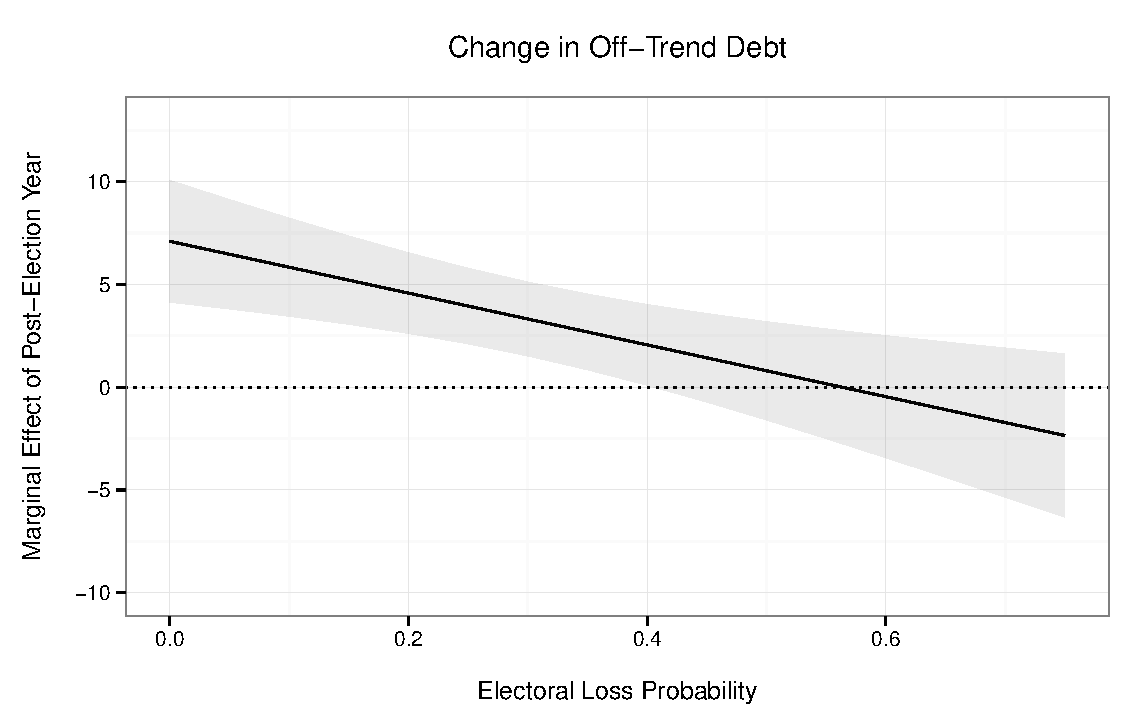
\includegraphics[scale=0.55]{figures/post_elect_loss.pdf}
    \end{center}

    {\scriptsize{Shaded area represents the 90\% confidence interval. \\
    Plot made using Model 5 in Table \ref{results_elect}.}}

\end{figure}

\subsection{Debt increases after elections}

We then examined how politician's electoral safety may affect changes to `off-trend' debt. To do this we created a dependent variable of the year-on-year change in the debt residuals. Table \ref{results_elect} shows results from partial correction panel models examining the relationship between electoral safety and changes to off-trend financial stress debt. Our primary covariate of interest is a post-election year dummy developed from Gandrud's \citeyearpar{gandrudYrcurnt} election timing variable. It is set at one in years following elections and zero otherwise. In addition, we are interested in electoral competitiveness as measured by the probability that the plurality party will lose its plurality in the next election. This variable is from \cite{Kayser2015comp}. In some specifications we included the governing party's economic ideology from \citep[][updated through 2012]{DPI2001}, a measure of political constraints from \cite[][updated through 2011]{Henisz2004},\footnote{We specifically used the POLCONIII variable.} a binary indicator of whether or not a country had a fixed foreign exchange regime, and an off-trend government economic policy spending indicator constructed in the same way as our off-trend debt indicator using spending data from the OECD.\footnote{Data was accessed through \url{https://data.oecd.org/} in June 2015.}

Across the various model specifications we found that off-trend debt from perceived financial market stress is estimated to increase in post-election years. We further interacted the post-election year variable with electoral loss probability and found that off-trend debt increases after elections especially occur in countries  when there is a lower electoral loss probability (see Figure \ref{post_loss_me}). At higher loss probabilities the positive effect becomes insignificantly different from zero, meaning that when there is a higher probability of losing in the next election that governments do not have higher off-trend debt increases.

These results indicate that the timing of marginal government debt increases in response to financial crises may indeed be endogenous to politicians' electioneering. Creating something of a financial crisis political budget cycle. Very safe politicians, i.e. those who have just won an election and are less likely to lose the next one, are more likely to make public the costs of responding to financial market stress.


\section{Conclusions}\label{conclusions}

We have introduced a novel continuous measure of perceived financial market stress--FinStress--, compared it to prior measures of financial crisis and instability, and provided one application showing how our continuous measure could be used in future research to examine fiscal decisions in response to financial crises. Unlike previous measures, FinStress does not focus exclusively on financial market stress that, in hindsight, was not dealt with effectively by policy-makers. This could allow future researchers to examine what policies were effective at preventing full blown crises and what political conditions were conducive to implementing these policies. Being an indicator of perceived and real-time stress, rather than post hoc evaluations similarly provides a much more relevant indicator for understanding policy-makers' decision-making process at the time. FinStress should be used instead of previous second-best measures of financial market stress by researchers aiming to understand why and how policy-makers respond to financial market stress.

Our work has implications for the wider research community as well. We have demonstrated how researchers could construct continuous indicators of other political and economic phenomenon using machine learning and text analysis. Once a text gathering and analysis ``pipeline'' \citep{Leek2015} has been developed and validated, researchers using this approach can quickly and cost effectively develop and update new indicators. This approach is especially useful in comparison to time-consuming, expensive, and irreproducible human coding techniques.

Ideally, we would like to re-examine previous research that has relied on prior measures of financial market stress. This is currently difficult because much of the previous literature is strongly dependent on crises in the pre-2000 period \citep[see][]{GandrudHallerberg2015}, which is outside of the period that we are currently able to construct FinStress. However, there are clearly future research projects that could undertake this work as more data becomes available.

\bibliographystyle{apsr}
\bibliography{main.bib}

\clearpage

\section*{Online Appendix}

%\subsection*{Predicting Measures of Financial Market Stress with Z-Scores}

\begin{table}
    \caption{Do Z-Scores Predict Perceived Financial Market Stress?}
    \label{epfms_z_regress}

    \begin{center}
        
% Table created by stargazer v.5.1 by Marek Hlavac, Harvard University. E-mail: hlavac at fas.harvard.edu
% Date and time: Mon, Jul 13, 2015 - 11:07:38
\begin{tabular}{@{\extracolsep{5pt}}lc} 
\\[-1.8ex]\hline 
\hline \\[-1.8ex] 
 & \multicolumn{1}{c}{\textit{Dependent variable:}} \\ 
\cline{2-2} 
\\[-1.8ex] & Annual Mean EPFMS \\ 
\hline \\[-1.8ex] 
 Annual Mean EPFMS (lag) & 0.339$^{***}$ \\ 
  & (0.023) \\ 
  & \\ 
 Z-Score (lag) & 0.0002 \\ 
  & (0.0004) \\ 
  & \\ 
\hline \\[-1.8ex] 
Fixed effects? & Yes \\ 
Observations & 1,464 \\ 
R$^{2}$ & 0.149 \\ 
Adjusted R$^{2}$ & 0.130 \\ 
F Statistic & 112.040$^{***}$ (df = 2; 1278) \\ 
\hline 
\hline \\[-1.8ex] 
\textit{Note:}  & \multicolumn{1}{r}{$^{*}$p$<$0.1; $^{**}$p$<$0.05; $^{***}$p$<$0.01} \\ 
\end{tabular} 

    \end{center}
\end{table}

%\subsection*{Selection of Literature Including Cross-Country Measures of Financial or Banking Market Crisis}

\begin{table}[H]
\caption{Selected Literature Review of Political Institutions and Financial
Crisis (Political Outcomes)}


\label{LitRevTable2}
\begin{center}

\vspace{0.5cm}
\scalebox{0.9}{
\begin{tabular}{ m{2.5cm} m{1.75cm} m{6.25cm} m{2.5cm} }
    \hline
    Work & Crisis Type & Key Arguments/Findings & Crisis Data Sources \\
    \hline\hline

    %%% Bernhard and Leblang
    \cite{Bernhard2008} & Currency crisis & - Changes in the probability that cabinets will collapse condition the probability of speculative attacks.

    - Higher probability of a speculative attack decreases the probability of calling strategic elections. & Own data aggregated from multiple sources \\[0.25cm]\hline

    %%% Chwieroth and Walter
    \cite{Chwieroth2013} & Banking crises &  - Probability of government survival during crises changed over time as expectations changed about what governments should do to respond.

    - Governments with more veto players after the inter-war period are treated more harshly by voters. & \cite{ReinhartRog2010} \\[0.25cm]\hline

    \cite{CrespoTenorio2014} & Banking crisis & - Increasing globalization weakens the accountability link between politicians and voters.

    - Incumbents in open capital economies are more likely to survive a crisis, than those in closed economies. & Own data aggregated from multiple sources. \\[0.25cm]\hline

    %%% Montinola
    \cite{Montinola2003} & Banking crisis & - IMF credits decrease the probability of resolving banking crises.

    - The decisiveness of a political regime significantly influences the probability of emerging from systemic distress, though this depends on whether the crisis is moderate or severe. & Own data aggregated from multiple sources \\[0.25cm]\hline

    %%% Pepinsky
    \cite{Pepinsky2012} & Banking crisis & - Two factors--incumbent governments' responsibility for the current crisis and their responsiveness to its domestic economic effects--shape the political effects of the global economic crisis. & \cite{Laeven2010} \\[0.25cm]\hline

    \hline
\end{tabular}

}
\end{center}
\end{table}

\begin{table}[H]
\caption{Selected Literature Review of Political Institutions and Financial
Crisis (Crisis Occurrence, Policy Choices/Policy Outcomes)}


\label{LitRevTable}
\begin{center}

\vspace{0.5cm}
{\tiny{
\begin{tabular}{ m{2.5cm} m{2cm} m{7cm} m{3cm}}
    \hline
    Work & Crisis Type & Key Arguments/Findings & Crisis Data Sources \\
    \hline\hline

    %%% Broz
    \cite{broz2013} & Banking crisis & - In OECD countries right-wing governments pursue policies that lead to financial instability. Voters respond to resulting crises by voting in left-wing governments. & \cite{Reinhart2009,Laeven2012} \\[0.25cm]\hline

    %%% Galasso
    \cite{galasso2014} & Financial and economic crises & - Governments respond to financial crises by increasing regulation. & Dummy based on OECD output gap below -3.4\% \\[0.25cm]\hline

    %%% Gandrud
    \cite{Gandrud2013,Gandrud2014} & Banking crises & - Best practice financial governance institutional designs are more likely to be adopted during crises when there is high uncertainty about policy choices and outcomes. & \cite{Laeven2008,ReinhartRog2010} \\[0.25cm]\hline

    %%% Ha and Kang
    \cite{ha2015} & - Banking crisis & Developing countries respond to crises with fiscal and monetary tightening, which was moderated by political constraints, left ideology governing parties, and up coming elections. & \cite{Laeven2008}. \\[0.25cm]\hline

    %%% Hallerberg Scart
    \cite{HallerbergScartForthcoming} & Banking, debt crises & - Banking crises reduce the probability of fiscal reforms, but the longer a crisis lasts and if it becomes a sovereign debt crisis the the probability of reform increases.

    - Countries with more personalistic voting are more likely to reform. & \cite{Laeven2012} for Latin American countries \\[0.25cm]\hline

    %%% Hallerberg Wehner
    \cite{Hallerberg2013} & Banking, currency, debt crises & - Some evidence that more technically competent ministers of finance are appointed during debt crises. Not much robust evidence for other effects of crisis on the technical competency of economic policy-makers. & \cite{Laeven2012}  \\[0.25cm]\hline

    %%% Hicken et al.
    \cite{Hicken2005} (2005) & Growth shocks & - The size of the winning coalition is positively associated with growth recoveries following forced devaluations. & Own data aggregated from multiple sources \\[0.25cm]\hline

    %%%% Keefer
    \cite{Keefer2007} & Banking crises & - Higher electoral competitiveness leads to faster and less costly crisis responses.

    - Checks and balances not associated with crisis policy choices or outcomes. & Modified \cite{Honohan2003} \\[0.25cm]\hline

    %%% Kleibl
    \cite{Kleibl2013} & Banking crisis & - Responses to regulatory failures are conditioned by the level of public ownership in the banking sector. & \cite{Laeven2010,Reinhart2009} for OECD countries \\[0.25cm]\hline

    %%% MacIntyre
    \cite{MacIntyre2001} & Financial crises & - U-shaped relationship between veto players and crisis outcomes & Own data aggregated from multiple sources \\[0.25cm]\hline

    %%% Reischmann
    \cite{reischmann2015} & Banking crises & - Creative accounting as measured by changes in the stock flow adjustment occurs more during financial crises, though effect may be swallowed up by the period fixed effects in his regressions as crises are highly correlated with time in his sample. & \cite{Laeven2012} \\[0.25cm]\hline

    %%% Rodrick
    \cite{Rodrick1999} & Growth shock & - Many veto players, if organized to manage conflicts, will result in more appropriate and quickly implemented crisis management policies. & Own data aggregated from multiple sources \\[0.25cm]\hline

    %%%% Rosas
    \cite{Rosas2006,Rosas2009} & Banking crisis & - Democratic regimes have fewer bailouts.

    - Central bank independence and transparency lead to fewer bailouts. & Modified \cite{Honohan2000} \\[0.25cm]\hline

    %%% Seiferling and Tareq
    \cite{seiferling2015} & Banking crisis & - Find advanced economies governments extend more loans and purchase more equities in temporarily insolvent firms during financial crisis than emerging market governments. & \cite{Laeven2010} via \cite{weber2012} \\[0.25cm]\hline

    %%% Satyanath
    \cite{Satayanath2006} & Banking crises & - Executives without `banking cronies' and that are not prevented from appointing their own bureaucrats by many veto players are more likely to have stringent financial regulation that prevents crises. & Case studies of 7 East Asian countries using own data \\[0.25cm]\hline

    %%% Wibbels and Roberts
    \cite{Wibbels2010} & Currency, growth, \& fiscal crises & - Unions and strong left parties are more associated with crises, though combined strong unions-left parties may alleviate inflationary crises. & Own data aggregated from multiple sources for 17 Latin American countries \\[0.25cm]\hline


    \hline
\end{tabular}

}}
\end{center}
\end{table}

\end{document}
